\documentclass[12pt, spanish]{article}
\usepackage[spanish]{babel}
\selectlanguage{spanish}
%\usepackage{natbib}
\usepackage{url}
\usepackage[utf8x]{inputenc}
\usepackage{graphicx}
\graphicspath{{images/}}
\usepackage{parskip}
\usepackage{fancyhdr}
\usepackage{vmargin}
\usepackage{multirow}
\usepackage{float}
\usepackage{chngpage}
\usepackage{enumitem}
\usepackage{forloop}


\usepackage{amsfonts}

\usepackage{subcaption}

\usepackage{hyperref}
\usepackage[
    type={CC},
    modifier={by-nc-sa},
    version={4.0},
]{doclicense}

\hypersetup{
    colorlinks=true,
    linkcolor=blue,
    filecolor=magenta,
    urlcolor=cyan,
}

% para codigo
\usepackage{listings}
\usepackage{xcolor}



%% configuración de listings

\definecolor{listing-background}{HTML}{F7F7F7}
\definecolor{listing-rule}{HTML}{B3B2B3}
\definecolor{listing-numbers}{HTML}{B3B2B3}
\definecolor{listing-text-color}{HTML}{000000}
\definecolor{listing-keyword}{HTML}{435489}
\definecolor{listing-identifier}{HTML}{435489}
\definecolor{listing-string}{HTML}{00999A}
\definecolor{listing-comment}{HTML}{8E8E8E}
\definecolor{listing-javadoc-comment}{HTML}{006CA9}

\lstdefinestyle{eisvogel_listing_style}{
  language         = python,
%$if(listings-disable-line-numbers)$
%  xleftmargin      = 0.6em,
%  framexleftmargin = 0.4em,
%$else$
  numbers          = left,
  xleftmargin      = 0em,
 framexleftmargin = 0em,
%$endif$
  backgroundcolor  = \color{listing-background},
  basicstyle       = \color{listing-text-color}\small\ttfamily{}\linespread{1.15}, % print whole listing small
  breaklines       = true,
  frame            = single,
  framesep         = 0.19em,
  rulecolor        = \color{listing-rule},
  frameround       = ffff,
  tabsize          = 4,
  numberstyle      = \color{listing-numbers},
  aboveskip        = 1.0em,
  belowskip        = 0.1em,
  abovecaptionskip = 0em,
  belowcaptionskip = 1.0em,
  keywordstyle     = \color{listing-keyword}\bfseries,
  classoffset      = 0,
  sensitive        = true,
  identifierstyle  = \color{listing-identifier},
  commentstyle     = \color{listing-comment},
  morecomment      = [s][\color{listing-javadoc-comment}]{/**}{*/},
  stringstyle      = \color{listing-string},
  showstringspaces = false,
  escapeinside     = {/*@}{@*/}, % Allow LaTeX inside these special comments
  literate         =
  {á}{{\'a}}1 {é}{{\'e}}1 {í}{{\'i}}1 {ó}{{\'o}}1 {ú}{{\'u}}1
  {Á}{{\'A}}1 {É}{{\'E}}1 {Í}{{\'I}}1 {Ó}{{\'O}}1 {Ú}{{\'U}}1
  {à}{{\`a}}1 {è}{{\'e}}1 {ì}{{\`i}}1 {ò}{{\`o}}1 {ù}{{\`u}}1
  {À}{{\`A}}1 {È}{{\'E}}1 {Ì}{{\`I}}1 {Ò}{{\`O}}1 {Ù}{{\`U}}1
  {ä}{{\"a}}1 {ë}{{\"e}}1 {ï}{{\"i}}1 {ö}{{\"o}}1 {ü}{{\"u}}1
  {Ä}{{\"A}}1 {Ë}{{\"E}}1 {Ï}{{\"I}}1 {Ö}{{\"O}}1 {Ü}{{\"U}}1
  {â}{{\^a}}1 {ê}{{\^e}}1 {î}{{\^i}}1 {ô}{{\^o}}1 {û}{{\^u}}1
  {Â}{{\^A}}1 {Ê}{{\^E}}1 {Î}{{\^I}}1 {Ô}{{\^O}}1 {Û}{{\^U}}1
  {œ}{{\oe}}1 {Œ}{{\OE}}1 {æ}{{\ae}}1 {Æ}{{\AE}}1 {ß}{{\ss}}1
  {ç}{{\c c}}1 {Ç}{{\c C}}1 {ø}{{\o}}1 {å}{{\r a}}1 {Å}{{\r A}}1
  {€}{{\EUR}}1 {£}{{\pounds}}1 {«}{{\guillemotleft}}1
  {»}{{\guillemotright}}1 {ñ}{{\~n}}1 {Ñ}{{\~N}}1 {¿}{{?`}}1
  {…}{{\ldots}}1 {≥}{{>=}}1 {≤}{{<=}}1 {„}{{\glqq}}1 {“}{{\grqq}}1
  {”}{{''}}1
}
\lstset{style=eisvogel_listing_style}


\usepackage[default]{sourcesanspro}

\setmarginsrb{2 cm}{1 cm}{2 cm}{2 cm}{1 cm}{1.5 cm}{1 cm}{1.5 cm}

\title{Práctica 2.\\
Tkinter y robótica.\hspace{0.05cm} }
\author{Antonio David Villegas Yeguas}
\date{\today}

\renewcommand*\contentsname{hola}

\makeatletter
\let\thetitle\@title
\let\theauthor\@author
\let\thedate\@date
\makeatother

\pagestyle{fancy}
\fancyhf{}
\rhead{\theauthor}
\lhead{\thetitle}
\cfoot{\thepage}

\begin{document}

%%%%%%%%%%%%%%%%%%%%%%%%%%%%%%%%%%%%%%%%%%%%%%%%%%%%%%%%%%%%%%%%%%%%%%%%%%%%%%%%%%%%%%%%%

\begin{titlepage}
    \centering
    \vspace*{0.3 cm}
    
\includegraphics[scale = 0.50]{ugr.png}\\[0.7 cm]
    %\textsc{\LARGE Universidad de Granada}\\[2.0 cm]
    \textsc{\large 4º CSI 2020/21 - Grupo 1}\\[0.5 cm]
    \textsc{\large Grado en Ingeniería Informática}\\[0.5 cm]
    \rule{\linewidth}{0.2 mm} \\[0.2 cm]
    { \huge \bfseries \thetitle}\\
    \rule{\linewidth}{0.2 mm} \\[1 cm]

    \begin{minipage}{0.4\textwidth}
        \begin{flushleft} \large
            \emph{Autor:}\\
            \theauthor\\
			 \emph{DNI:}\\
            77021623-M
            \end{flushleft}
            \end{minipage}~
            \begin{minipage}{0.4\textwidth}
            \begin{flushright} \large
            \emph{Asignatura: \\
            Programación Técnica y Científica}   \\
            \emph{Correo:}\\
            advy99@correo.ugr.es
        \end{flushright}
    \end{minipage}\\[0.5cm]

    {\large \thedate}\\[0.5cm]
    %{\url{https://github.com/advy99/AA/}}
    {\doclicenseThis}

    \vfill

\end{titlepage}

%%%%%%%%%%%%%%%%%%%%%%%%%%%%%%%%%%%%%%%%%%%%%%%%%%%%%%%%%%%%%%%%%%%%%%%%%%%%%%%%%%%%%%%%%

\tableofcontents
\pagebreak

%%%%%%%%%%%%%%%%%%%%%%%%%%%%%%%%%%%%%%%%%%%%%%%%%%%%%%%%%%%%%%%%%%%%%%%%%%%%%%%%%%%%%%%%%


\section*{Introducción}

En esta práctica trabajaremos con el módulo Tkinter para crear interfaces de usuario, con la herramienta V-REP de Coppelia Robotics AG en la que simularemos una escena con un robot para tomar datos, los cuales procesaremos en nuestra aplicación de cara a realizar aprendizaje automático y ser capaces de detectar una clase concreta de objetos de V-REP.

\section{Apartados realizados}

He realizado todos los apartados, tanto la interfaz de usuario como los módulos capturar, agrupar, características, clasificarSVM y predecir. A continuación explicaré como he ido realizando cada módulo y añadiré algunas imágenes de ejemplos tomados. 

\section{Desarrollo de la interfaz: mainInterfaz}

De cara a desarrollar la interfaz he seguido los pasos explicados en el guión con los conocimientos adquiridos en teoría sobre Tkinter.

La interfaz inicial se separa en cuatro columnas, con distintas filas para agrupar en grid los distintos textos, botones, cuadros de entrada y de selección.

\begin{figure}[H]
    \centering
    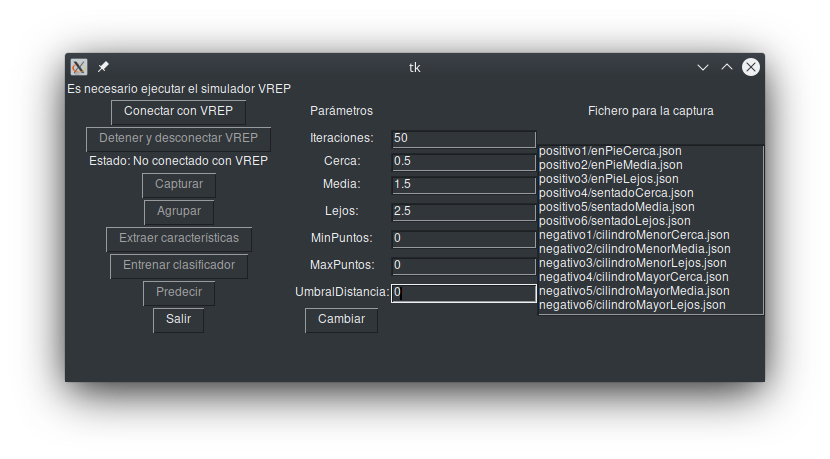
\includegraphics[width=\textwidth]{interfaz_vacia.png}
    \caption{Imagen inicial de la interfaz.}
\end{figure}

De cara a las distintas operaciones se ha utilizado mensajes de error, avisos y preguntas de si/no, tal y como se pedía en el guión de prácticas.

\begin{figure}[H]
    \centering
    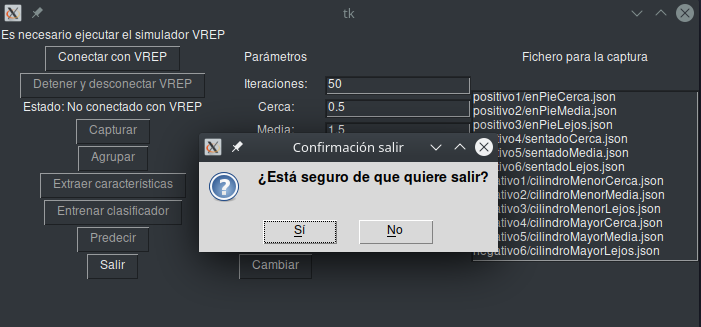
\includegraphics[width=\textwidth]{pregunta_salida.png}
    \caption{Confirmación salida.}
\end{figure}

\begin{figure}[H]
    \centering
    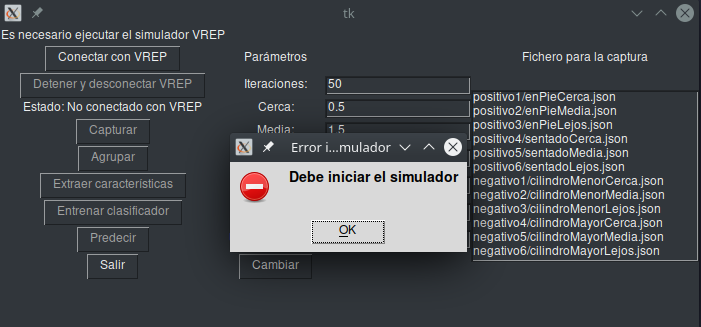
\includegraphics[width=\textwidth]{intento_conexion.png}
    \caption{Intento de conexión sin iniciar el simulador.}
\end{figure}

\begin{figure}[H]
    \centering
    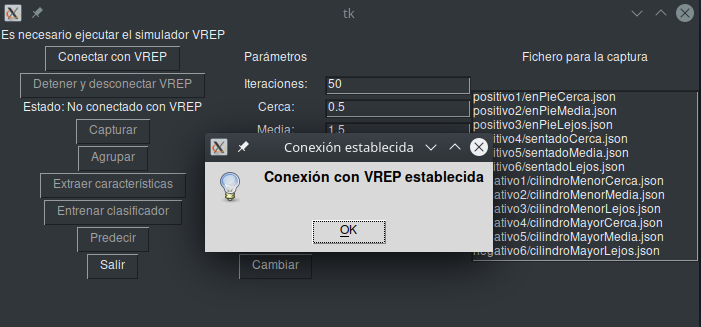
\includegraphics[width=\textwidth]{conexion.png}
    \caption{Conexión con el simulador.}
\end{figure}

\begin{figure}[H]
    \centering
    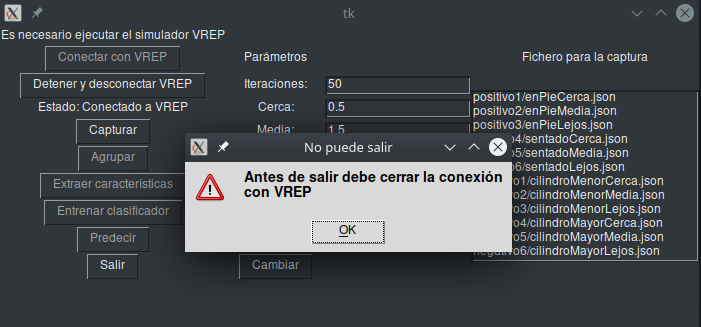
\includegraphics[width=\textwidth]{intento_salida.png}
    \caption{Intento de salida con el simulador conectado.}
\end{figure}

\begin{figure}[H]
    \centering
    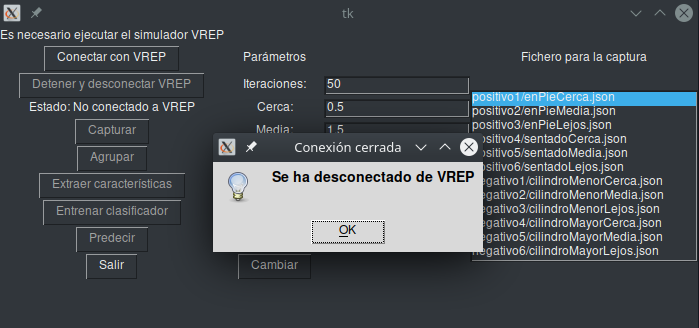
\includegraphics[width=\textwidth]{detener_vrep.png}
    \caption{Desconexión con el simulador.}
\end{figure}

\begin{figure}[H]
    \centering
    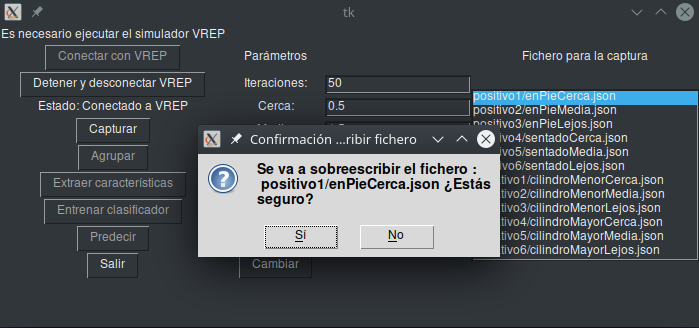
\includegraphics[width=\textwidth]{creacion_capturar.png}
    \caption{Aviso sobreescribir al capturar.}
\end{figure}

\begin{figure}[H]
    \centering
    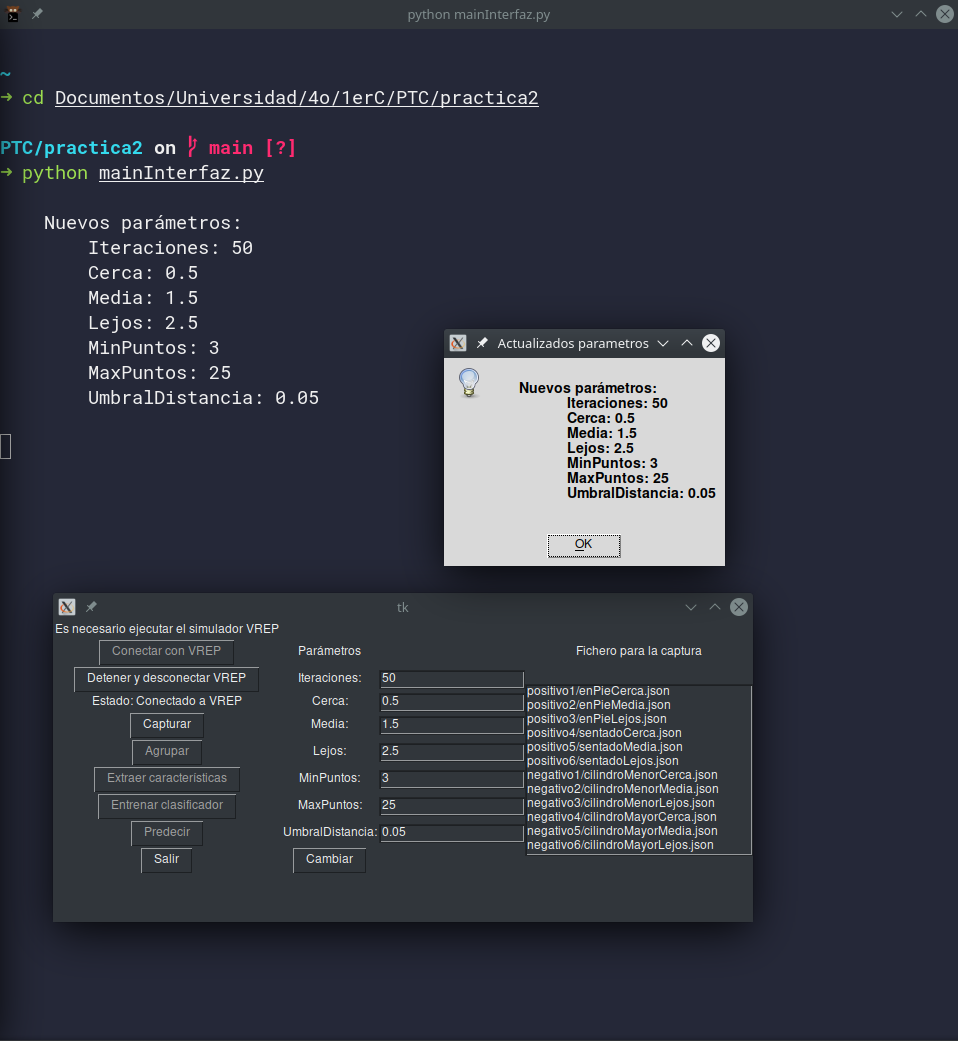
\includegraphics[width=\textwidth]{cambio_parametros.png}
    \caption{Avisos al cambiar los parámetros.}
\end{figure}

Los distintos botones tienen asociadas funciones dentro del \texttt{mainInterfaz}, que irán haciendo llamadas a los correspondientes módulos explicados más adelante, así como activando otros botones según se trabaja.

Cuando nos conectamos con el simulador V-REP activamos el botón para capturar, y a su vez, cuando capturamos los doce archivos activamos el botón agrupar. Esto se ha hecho insertando en una lista los nombres de los ficheros, y comprobando que el número de elementos sin repeticiones fuera doce.


\begin{figure}[H]
    \centering
    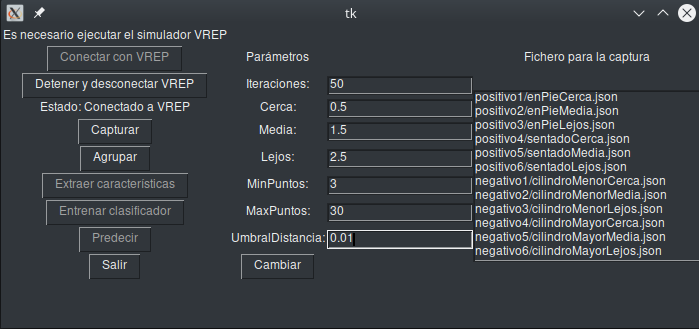
\includegraphics[width=\textwidth]{boton_agrupar_activo.png}
    \caption{Activación del boton agrupar.}
\end{figure}

Una vez agrupamos los datos en los clusters, se activará el botón extraer características.


\begin{figure}[H]
    \centering
    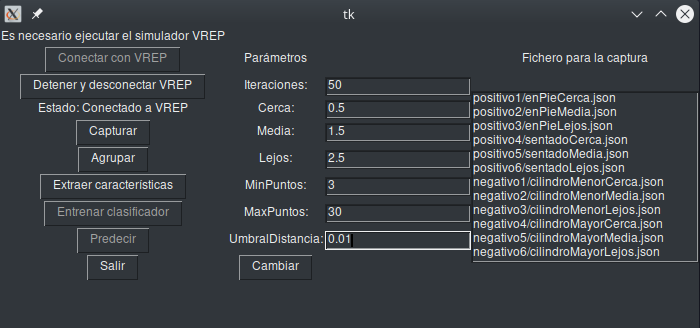
\includegraphics[width=\textwidth]{boton_extraer_c.png}
    \caption{Activación del boton extraer características.}
\end{figure}

Tras extraer las características se activará el boton para entrenar el clasificador.

\begin{figure}[H]
    \centering
    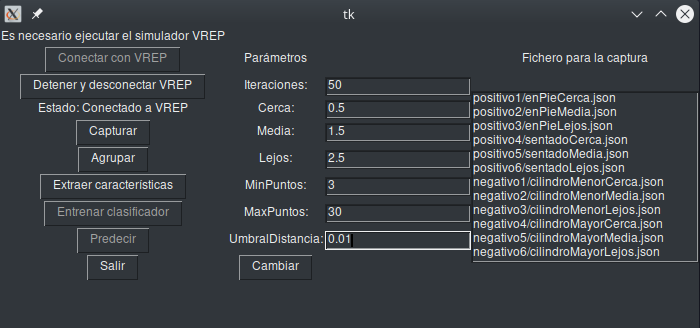
\includegraphics[width=\textwidth]{boton_extraer_c.png}
    \caption{Activación del boton entrenar clasificador.}
\end{figure}

Al entrenar el clasificador podremos predecir una nueva escena con todos los tipos.

\begin{figure}[H]
    \centering
    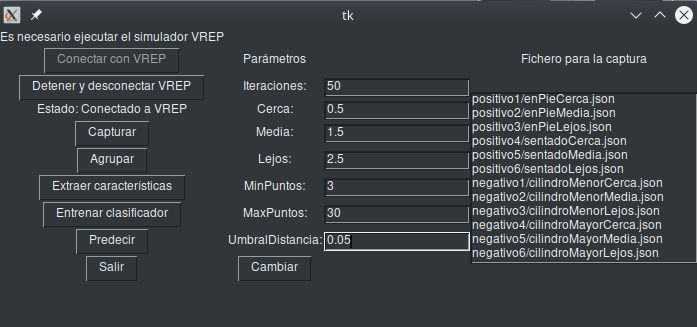
\includegraphics[width=\textwidth]{boton_predecir.png}
    \caption{Activación del boton predecir.}
\end{figure}


\section{Desarrollo del módulo capturar}

Este módulo simplemente se conectará con V-REP y tomará datos leidos por el laser. Este módulo se ha desarrollado en distintas funciones de cara a reutilizarlas para leer tanto los casos positivos como los negativos, además de las escenas que tengamos que predecir.

\section{Desarrollo del módulo agrupar}

En este módulo encontraremos varias funciones. La principal es, dada una muestra, agrupará en clusters los puntos de dicha muestra con el algoritmo dado en el guión. Esta función se usará tanto para la muestra de la escena de test, como para las escenas capturadas en los módulos anteriores. Para esto se han desarrollado distintas funciones para dada una lista de ficheros calcular los clusters de las muestras de dichos ficheros, así como para dado una serie de clusters volcarlos a un fichero como se nos pide en el guión.

\section{Desarrollo del módulo caracteristicas}

El módulo características cuenta con tres funciones para calcular las distintas carácterísticas que se piden, además de la función principal y otra función que generará el csv pedido que se utilizará más adelante.

\section{Desarrollo del módulo clasificarSVM}

Este módulo carga el csv generado por el módulo características y ajustará tres clasificadores SVC distintos kernels y parámetros para estos datos. De cara a la búsqueda de parámetros óptimos se ha utilizado GridSearchCV y se compararán los clasificadores con su valoración de validación cruzada con cinco folds, de cara a comprobar que el funcionamiento del clasificador es correcto.

\section{Desarrollo del módulo predecir}

Para predecir simplemente utilizaremos los módulos anteriores para capturar datos de la escena que queremos predecir, los agruparemos en clusters, calcularemos sus características y utilizaremos el clasificador entrenado en el apartado anterior para predecir la clase de cada cluster. Como salida generará una imagen con los clusters obtenidos, en rojo los que considera piernas, y en azul los que no.


\section{Funcionamiento}

El funcionamiento de la aplicación es sencillo, una vez lanzada la interfaz, capturamos los datos con los parámetros que consideremos, agrupamos los datos capturados de entrenamiento, calculamos sus características, entrenamos el modelo, y eso nos permitirá predecir nuevas escenas. Todo esto lo podemos hacer con la interfaz creada.

\subsection{Parámetros usados}

He utilizado los siguientes parámetros:

\begin{itemize}
    \item Iteraciones: 50
    \item Cerca: 0.5
    \item Media: 1.5
    \item Lejos: 2.5
    \item MinPuntos: 3
    \item MaxPuntos: 30
    \item UmbralDistancia: 0.01
\end{itemize}

Estos parámetros los he escogido porque empíricamente han funcionado bien y han dado buenos resultados tras haber probado con otros en comparación. También algunos, como por ejemplo MinPuntos, se han escogido con un mínimo de tres, ya que si no no podríamos extraer características en tres dimensiones de los clusters, o UmbralDistancia se ha escogido un umbral muy bajo, ya que al ir realizando pruebas de agrupamiento los puntos estaban muy cerca.

\subsection{Capturas de datos}

\begin{figure}[H]
    \centering
    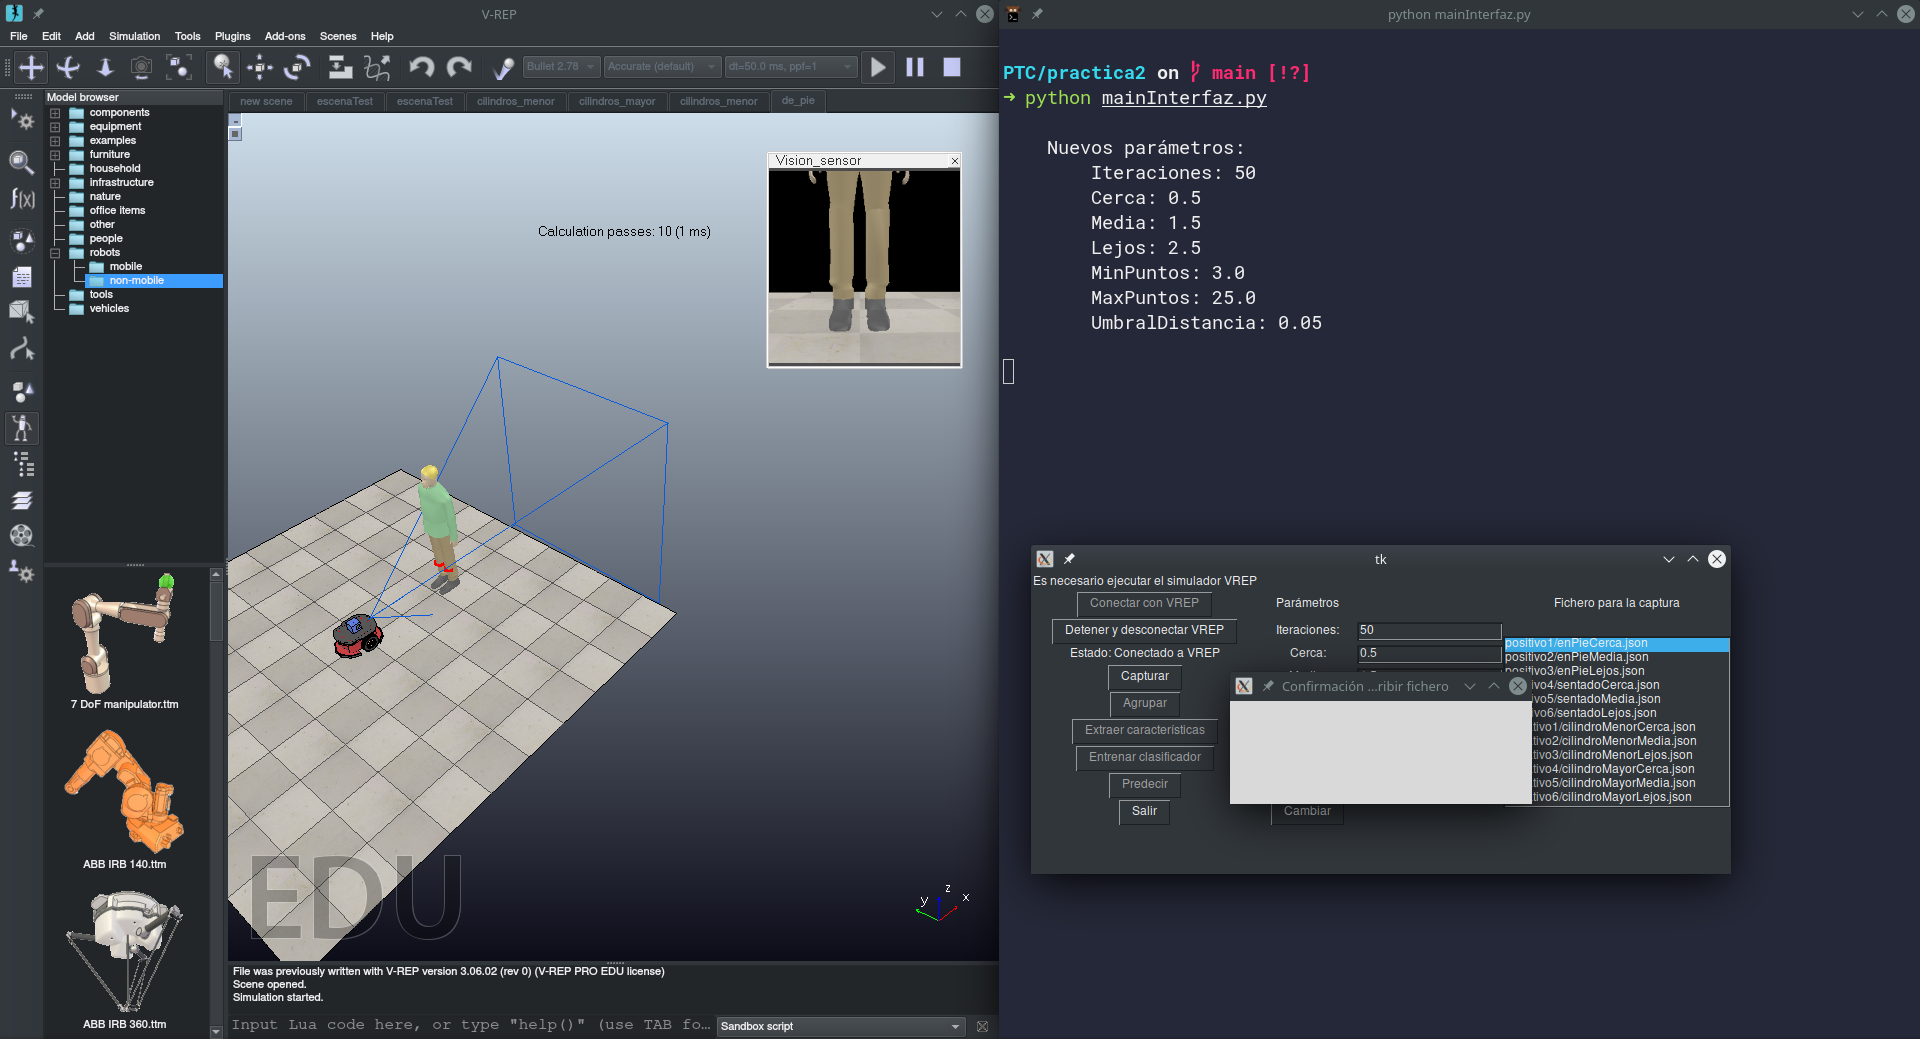
\includegraphics[width=\textwidth]{captura_datos.png}
    \caption{Captura de datos con Bill de pie cerca.}
\end{figure}

\begin{figure}[H]
    \centering
    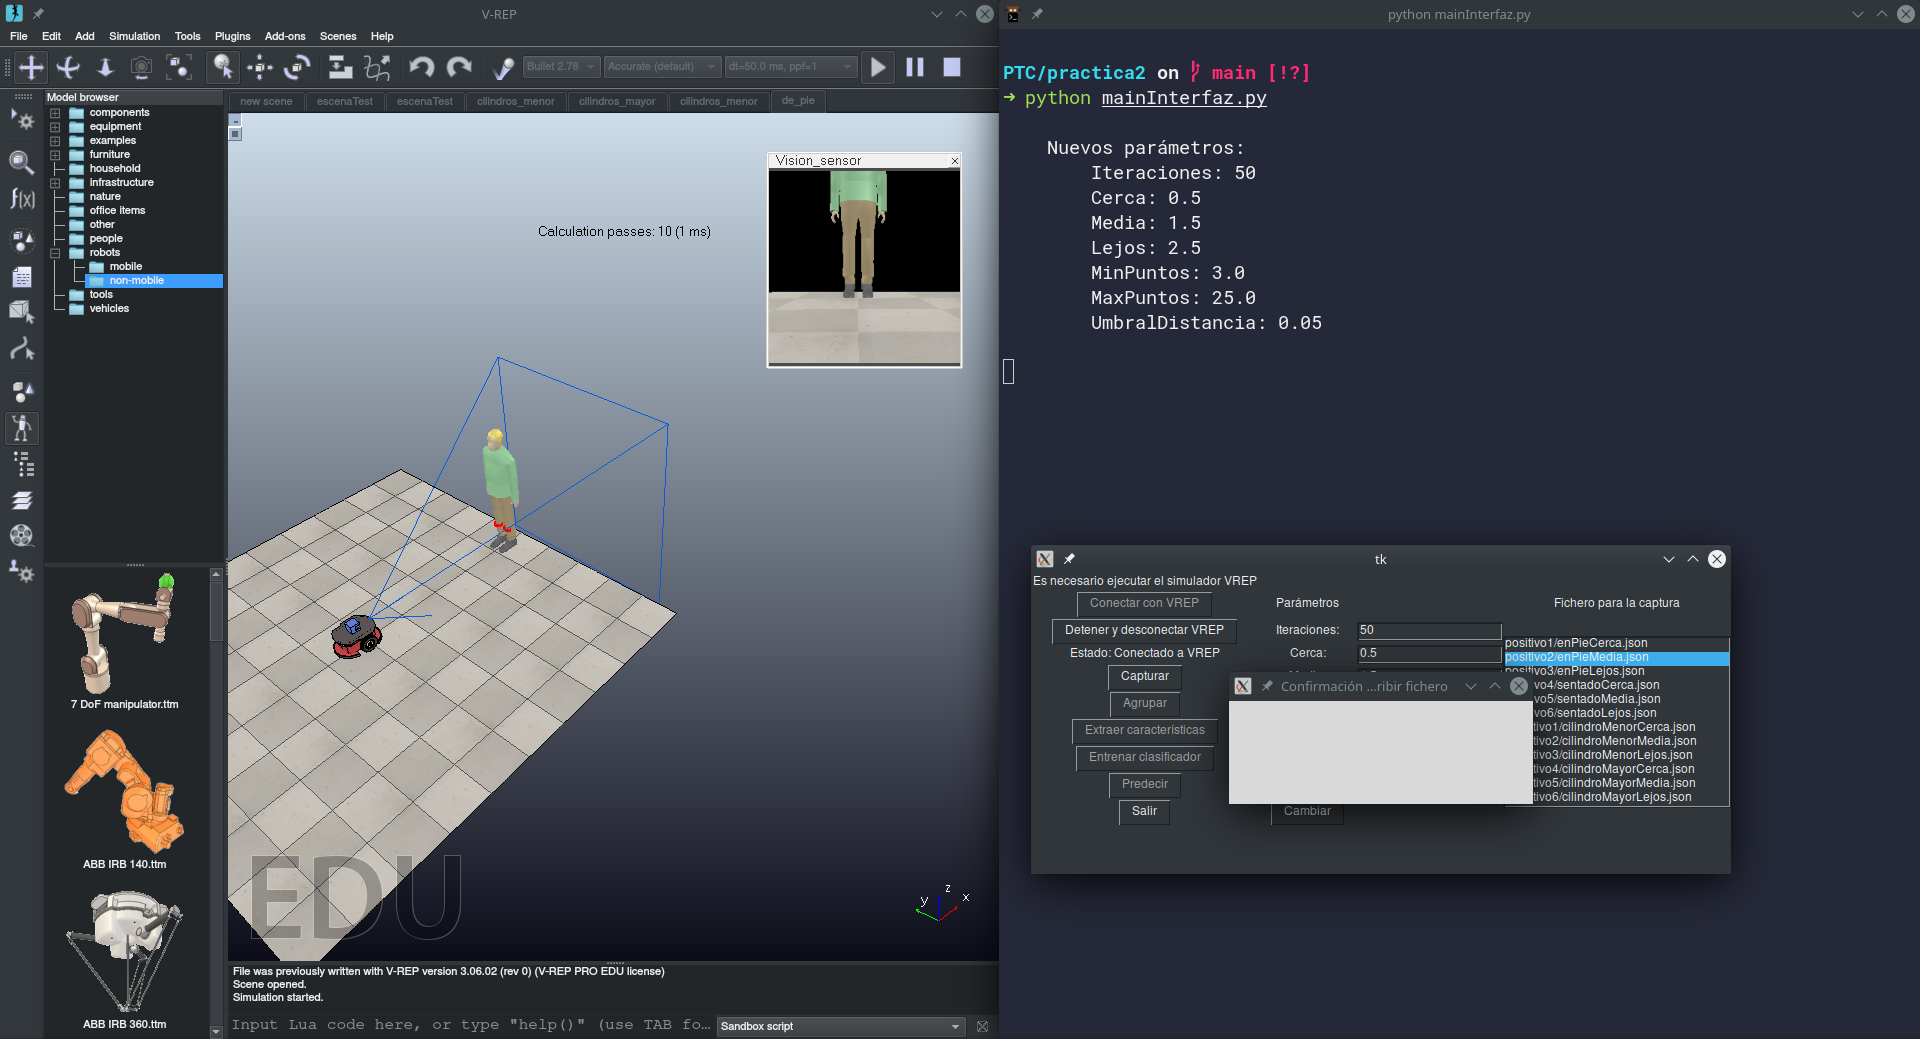
\includegraphics[width=\textwidth]{captura_media.png}
    \caption{Captura de datos con Bill de pie media.}
\end{figure}

\begin{figure}[H]
    \centering
    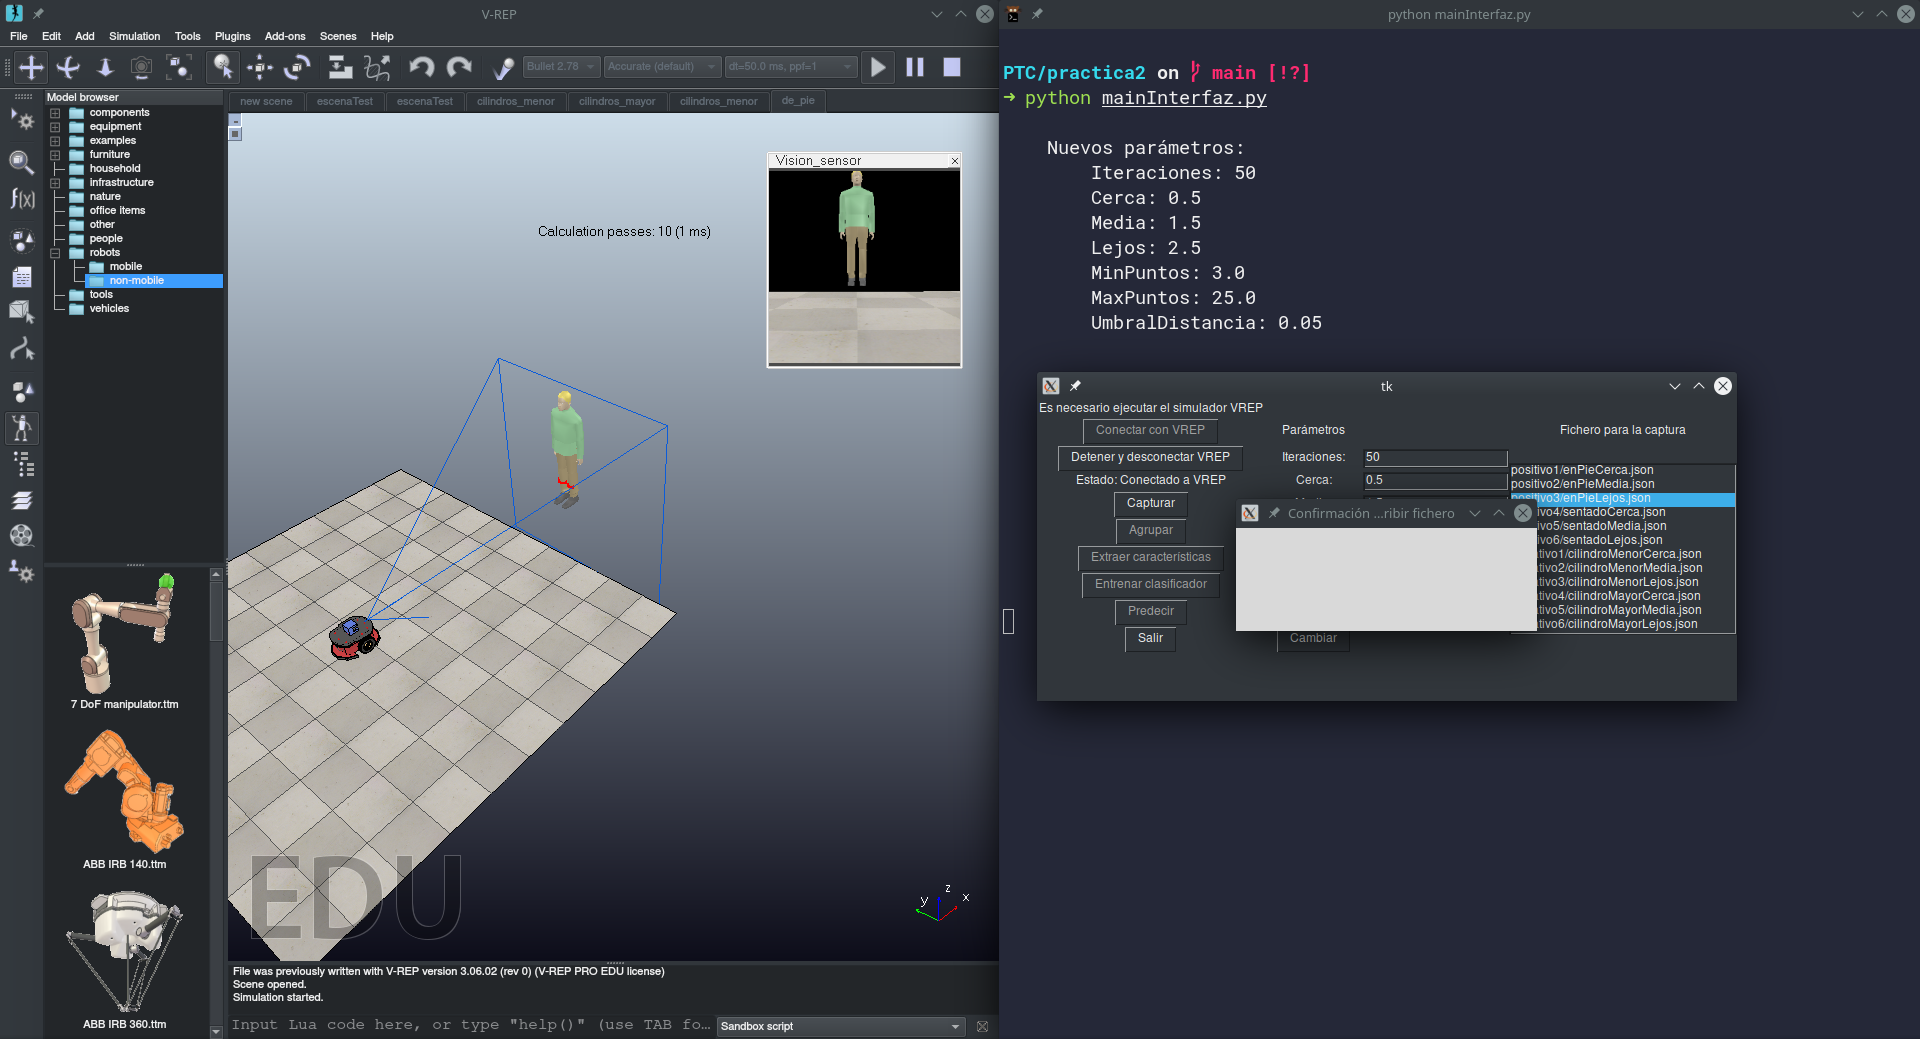
\includegraphics[width=\textwidth]{captura_lejos.png}
    \caption{Captura de datos con Bill de pie lejos.}
\end{figure}

\begin{figure}[H]
    \centering
    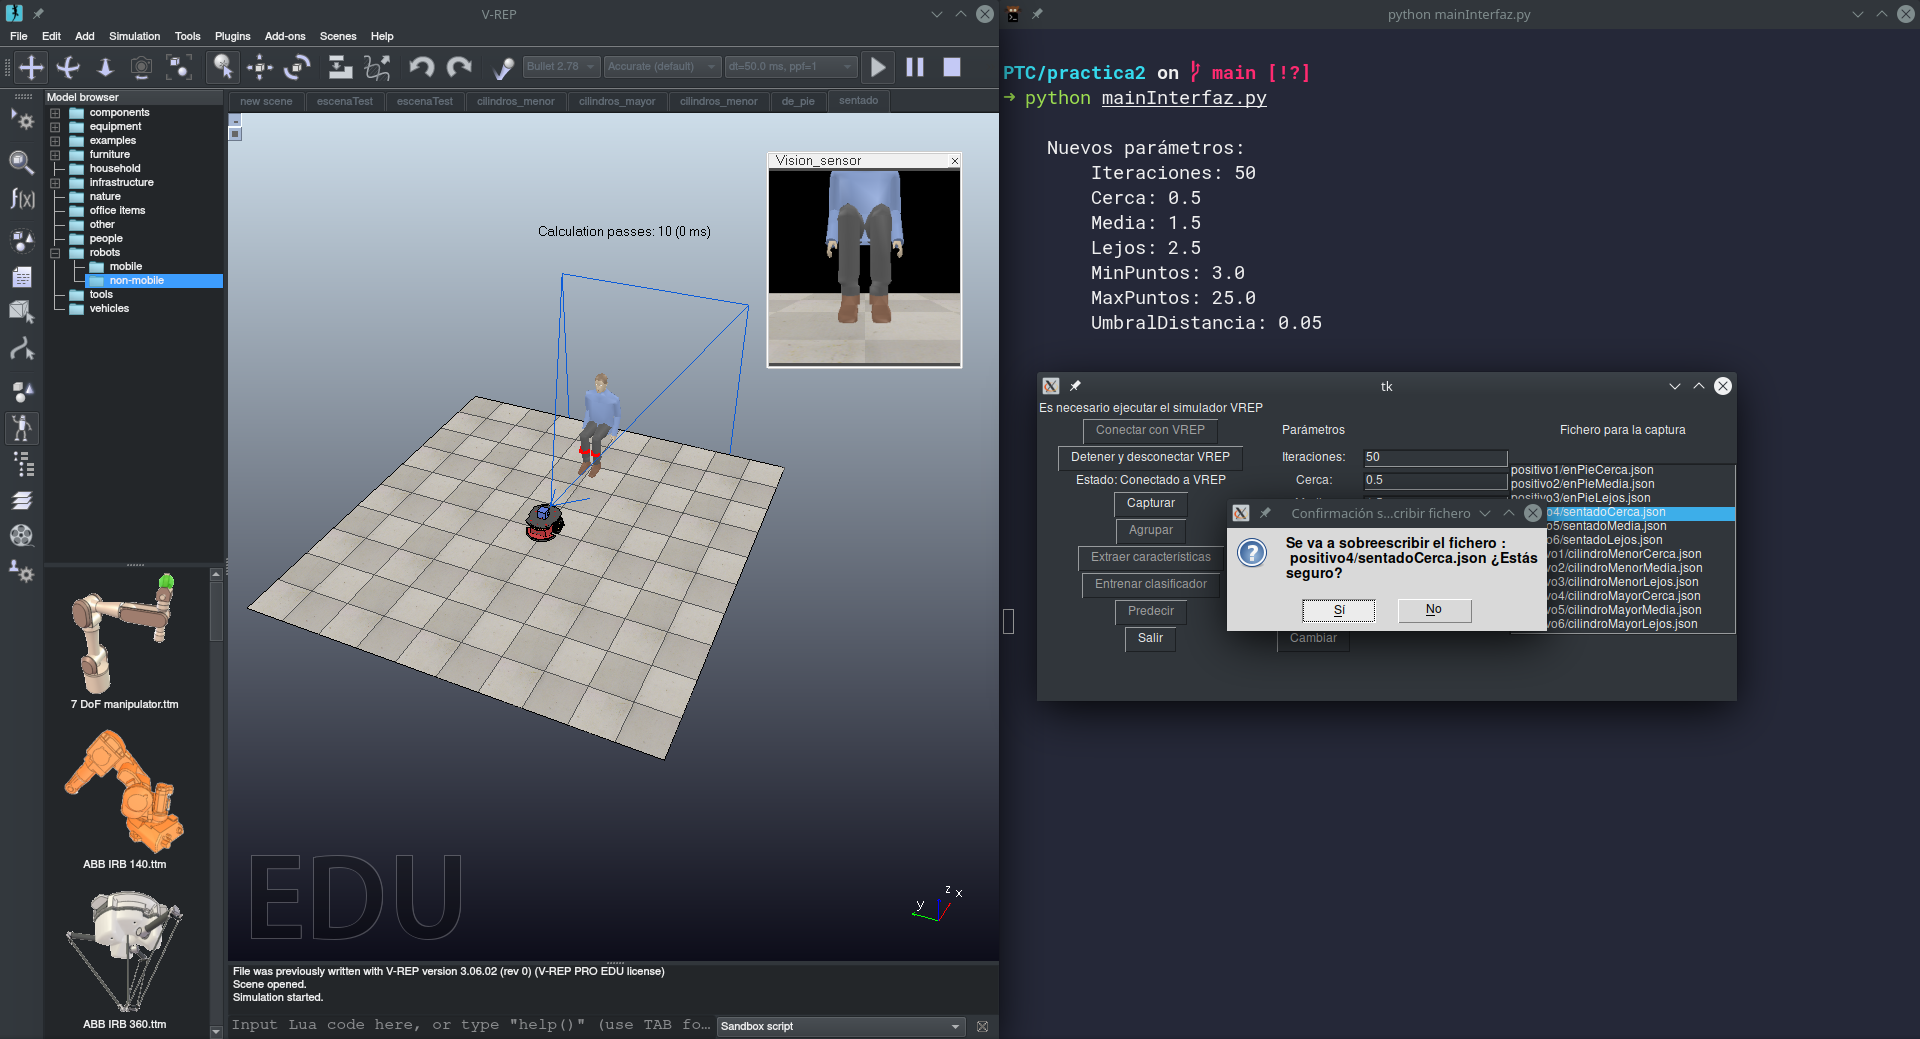
\includegraphics[width=\textwidth]{sentado_cerca.png}
    \caption{Captura de datos con Bill sentado cerca.}
\end{figure}

\begin{figure}[H]
    \centering
    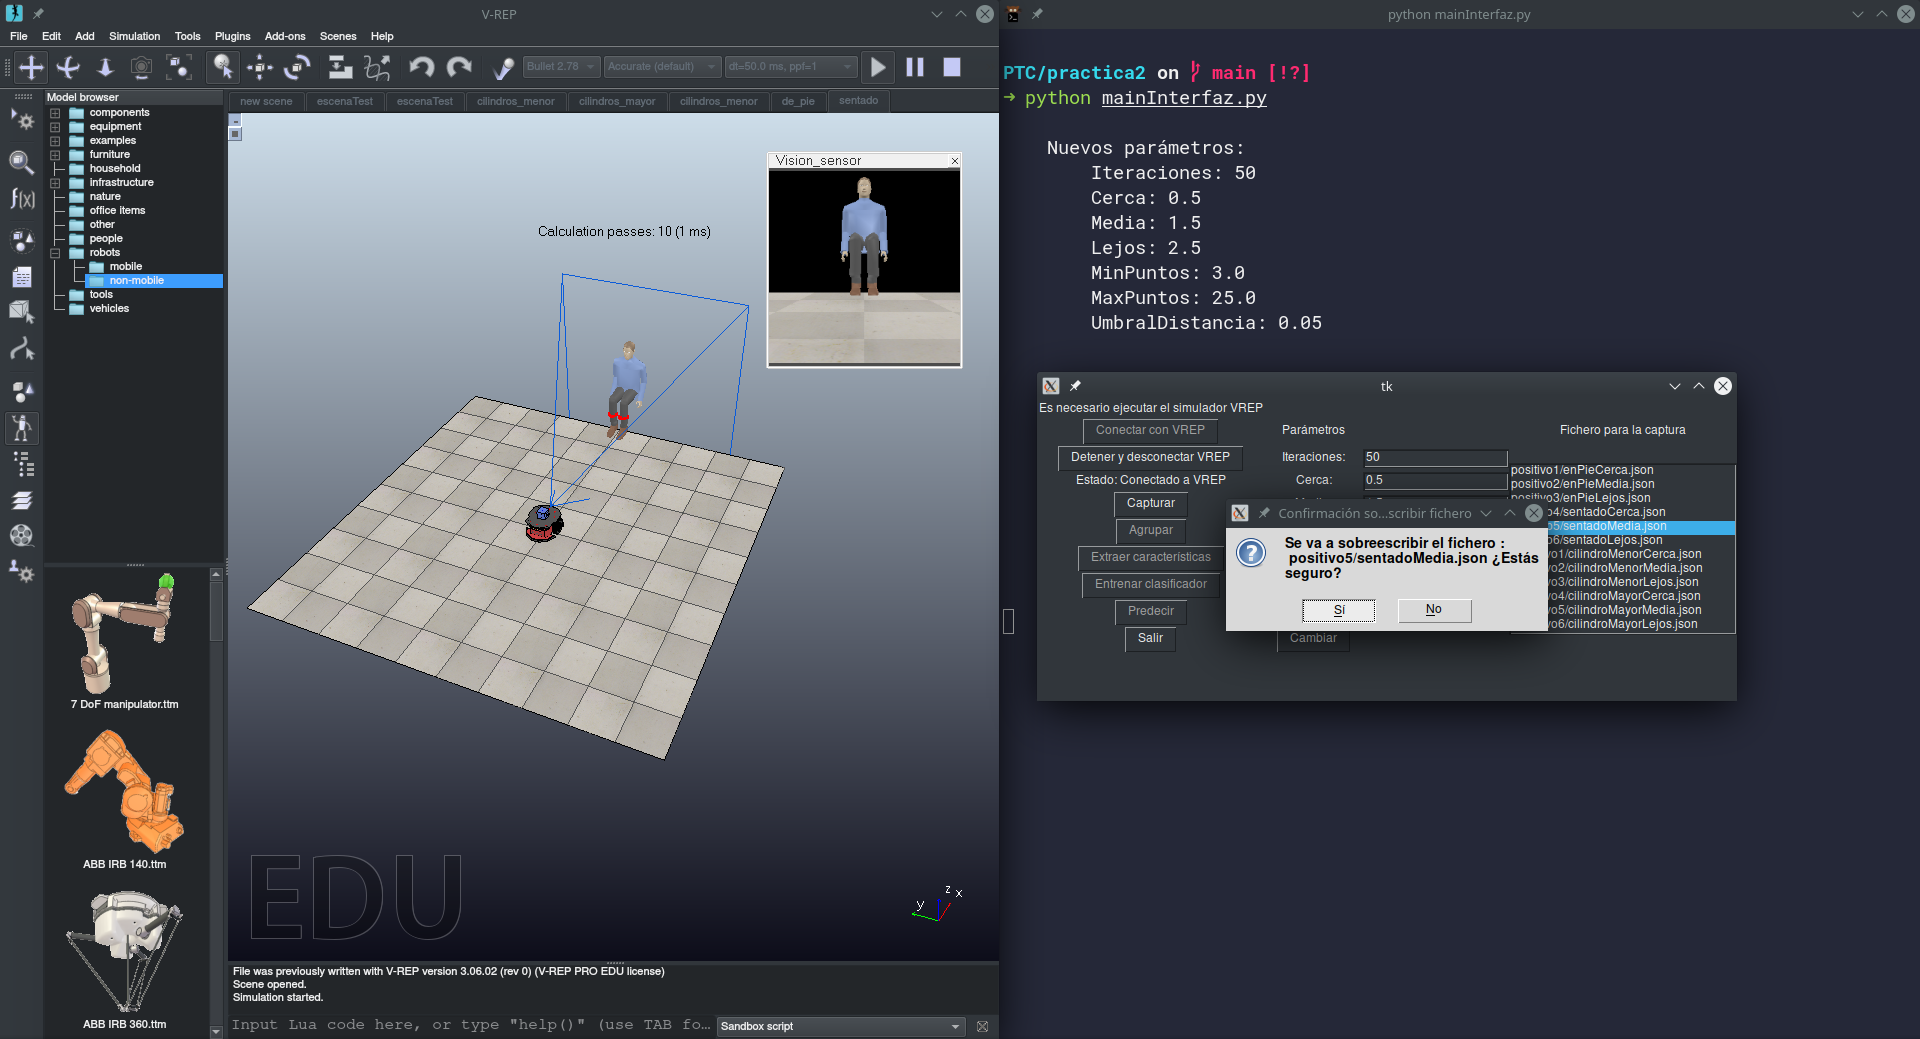
\includegraphics[width=\textwidth]{sentado_media.png}
    \caption{Captura de datos con Bill sentado media.}
\end{figure}

\begin{figure}[H]
    \centering
    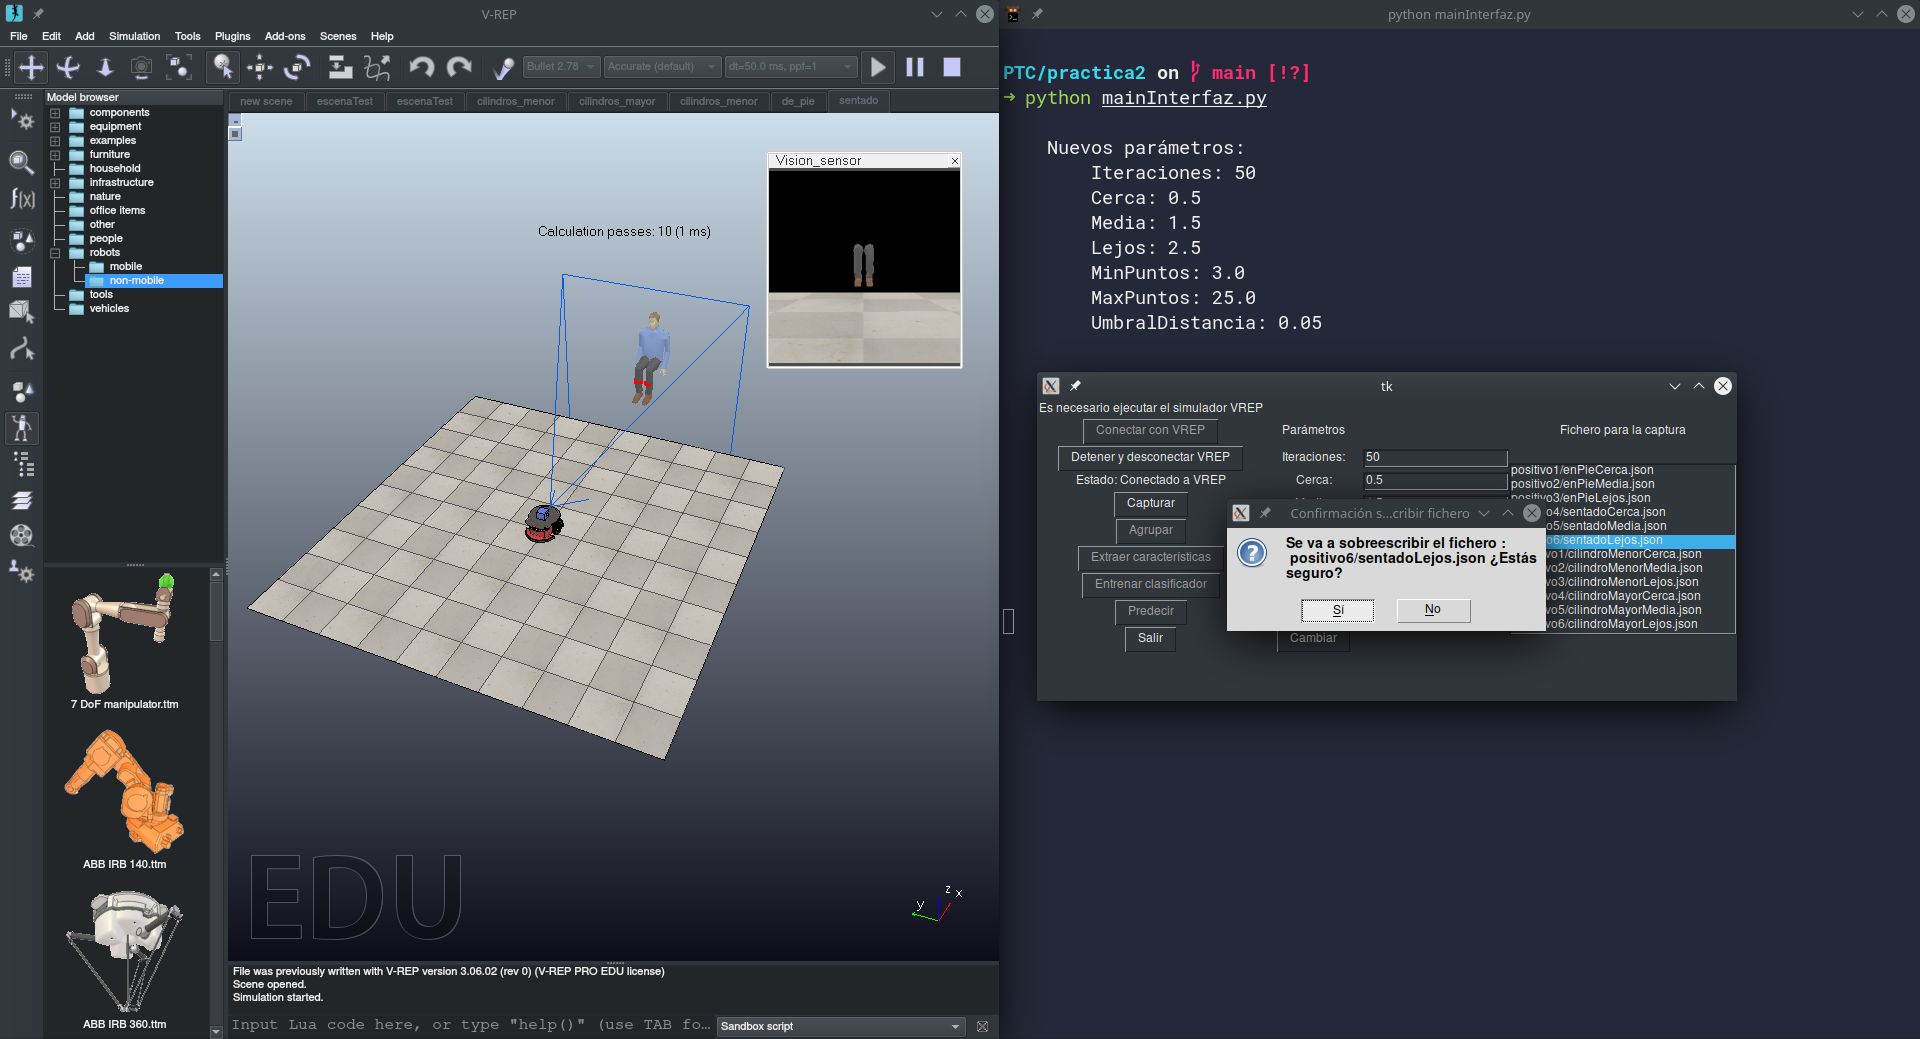
\includegraphics[width=\textwidth]{sentado_lejos.png}
    \caption{Captura de datos con Bill sentado lejos.}
\end{figure}





\begin{figure}[H]
    \centering
    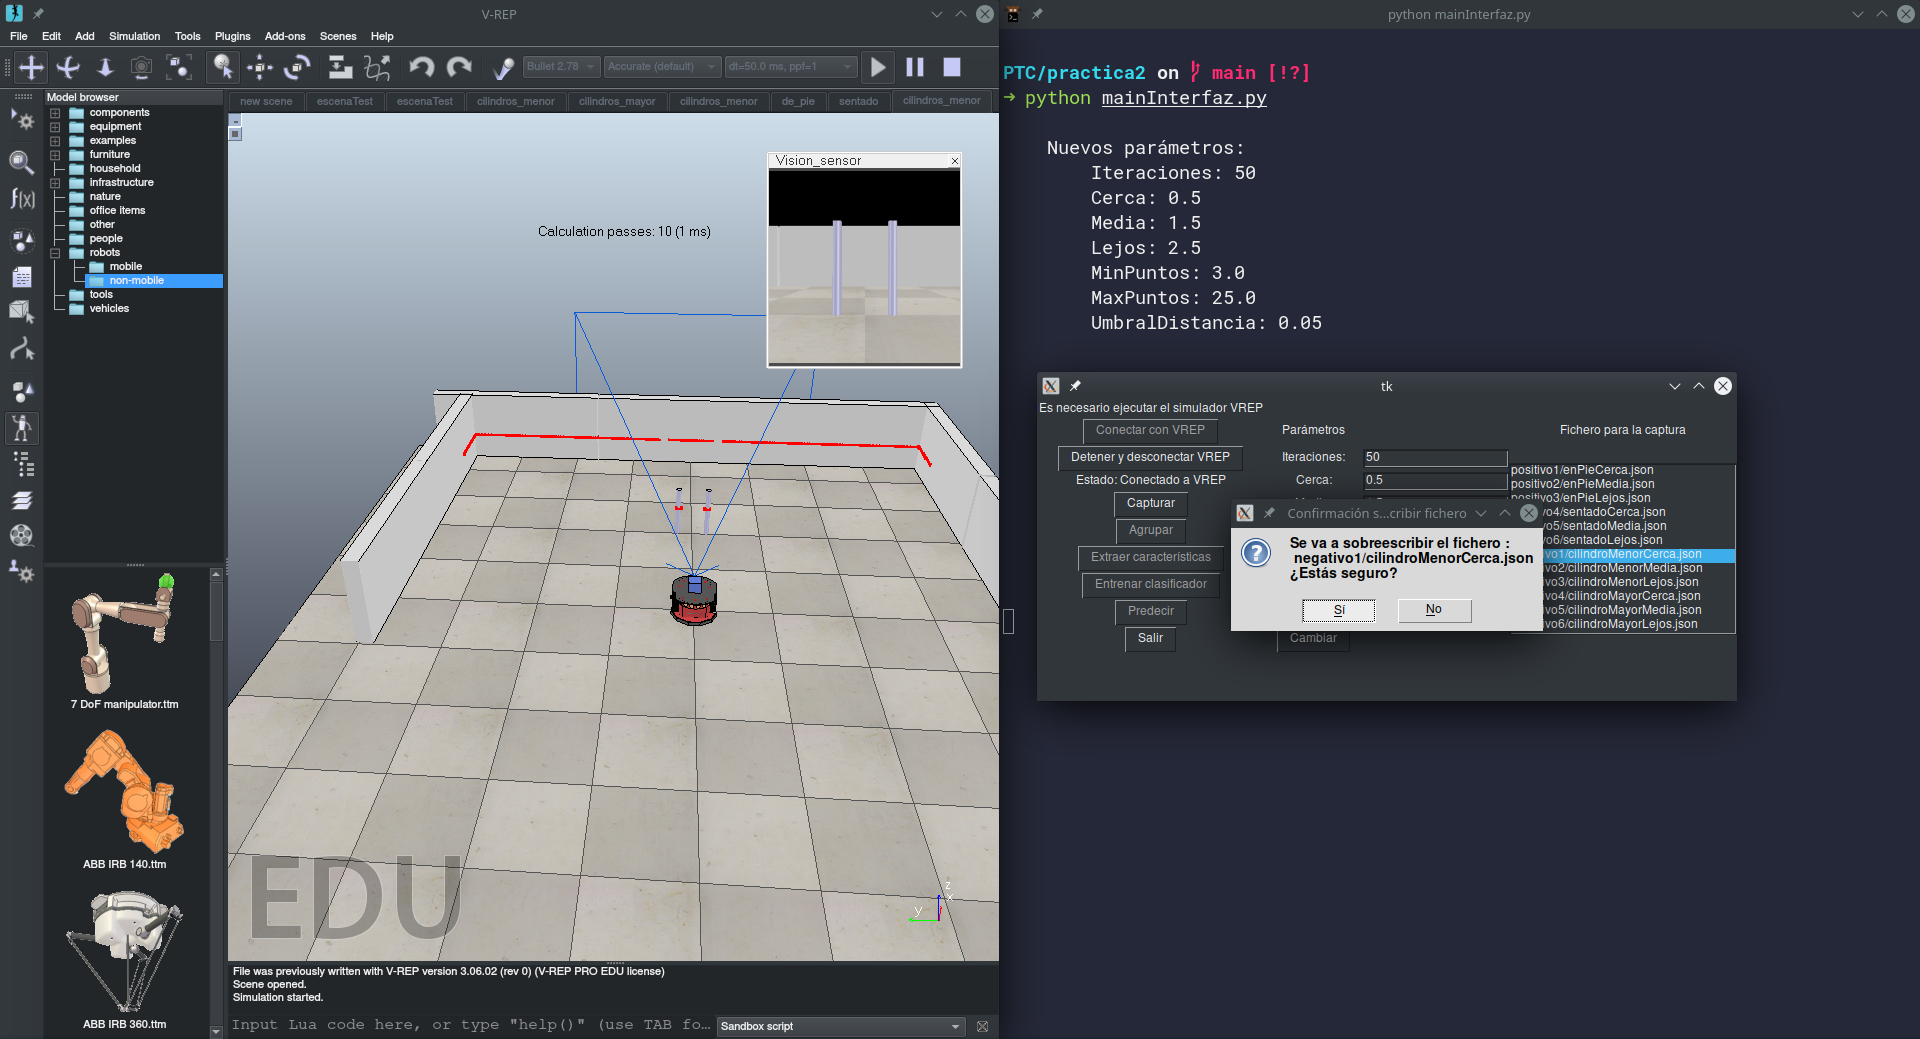
\includegraphics[width=\textwidth]{cilindro_p_cerca.png}
    \caption{Captura de datos con cilindro pequeño cerca.}
\end{figure}

\begin{figure}[H]
    \centering
    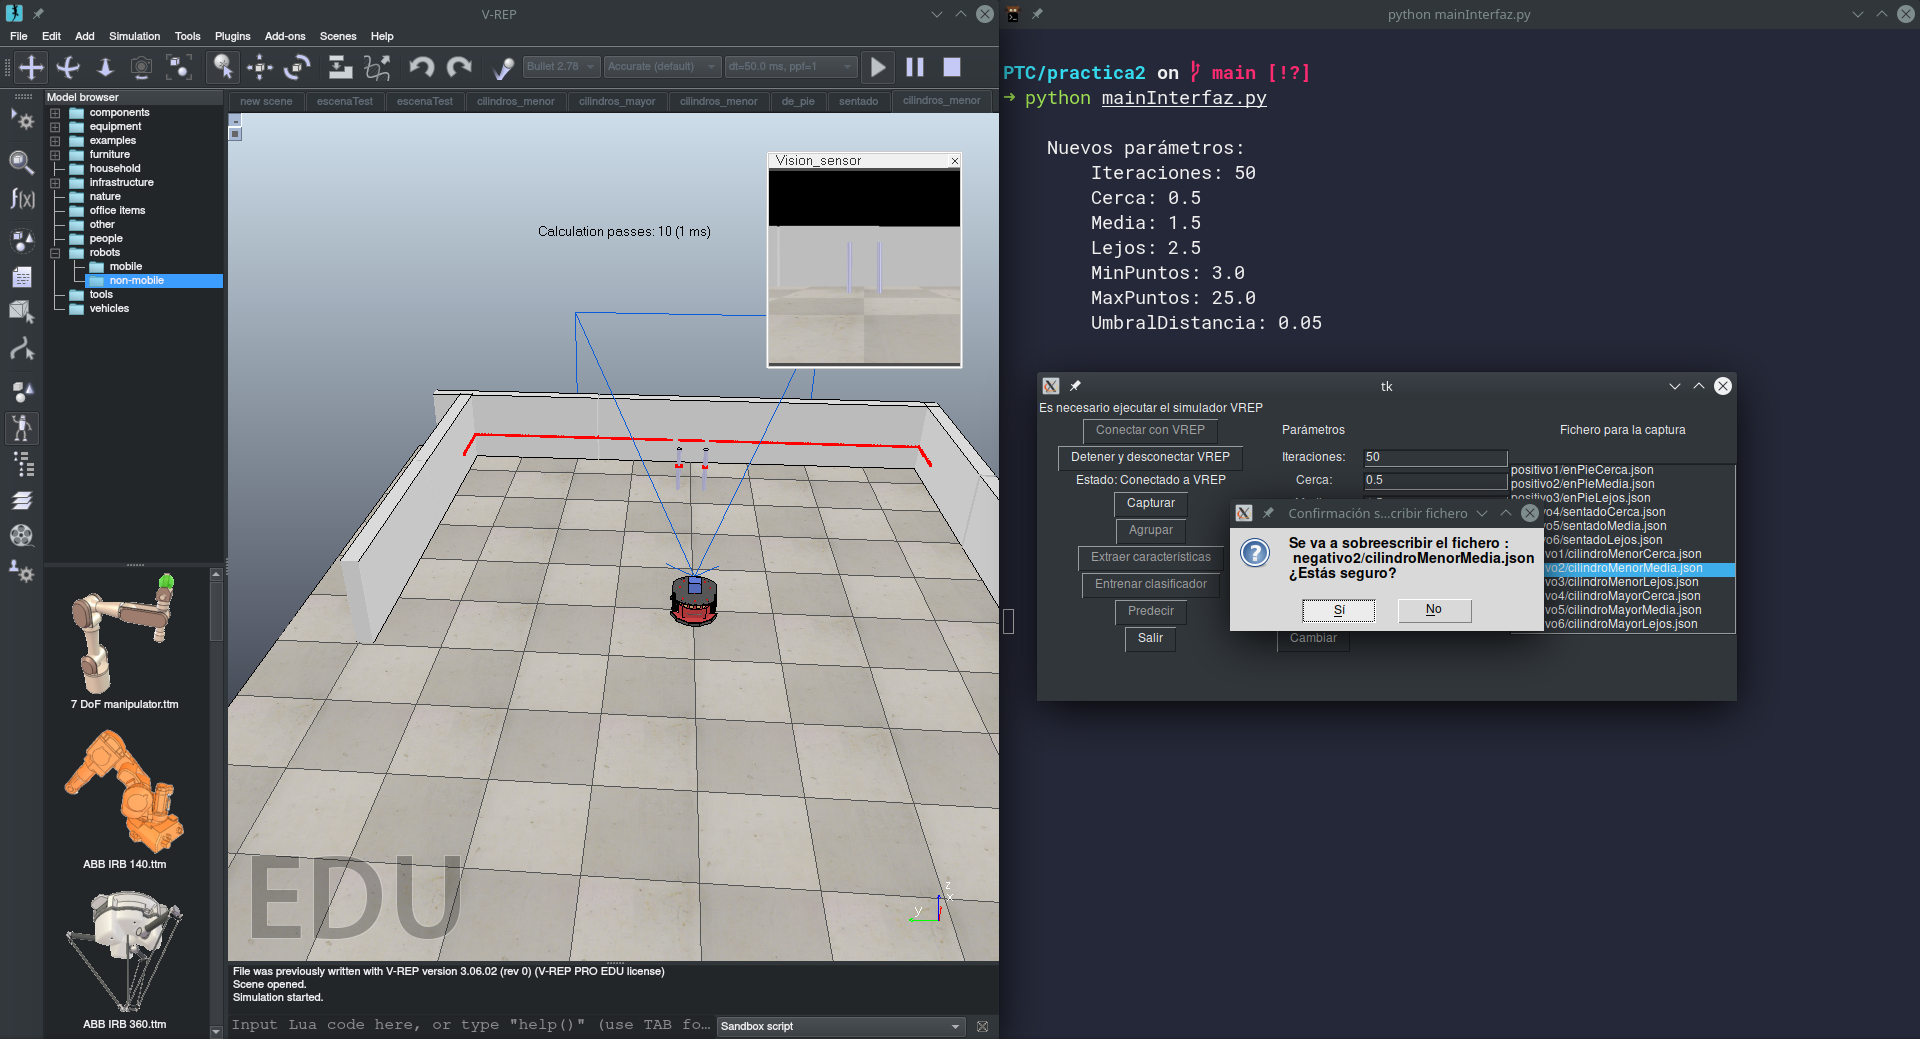
\includegraphics[width=\textwidth]{cilindro_p_media.png}
    \caption{Captura de datos con cilindro pequeño media.}
\end{figure}

\begin{figure}[H]
    \centering
    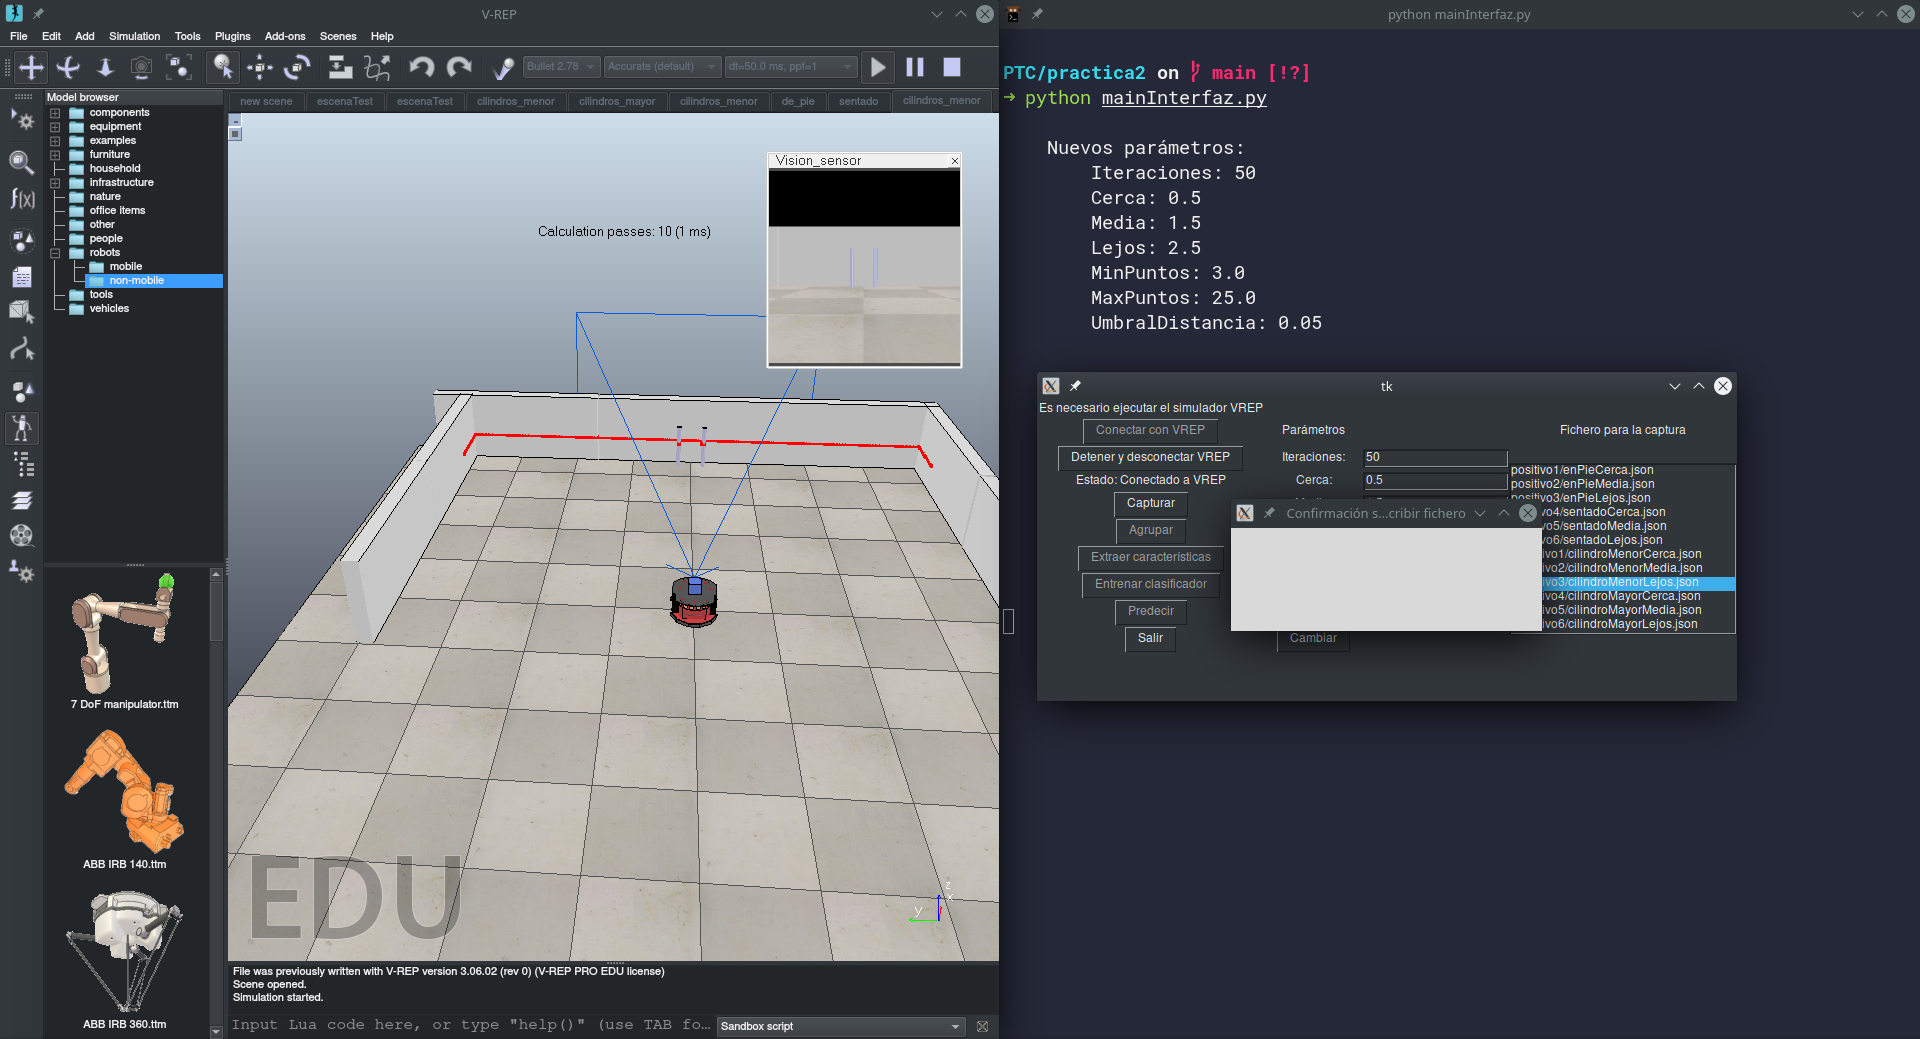
\includegraphics[width=\textwidth]{cilindro_p_lejos.png}
    \caption{Captura de datos con cilindro pequeño lejos.}
\end{figure}

\begin{figure}[H]
    \centering
    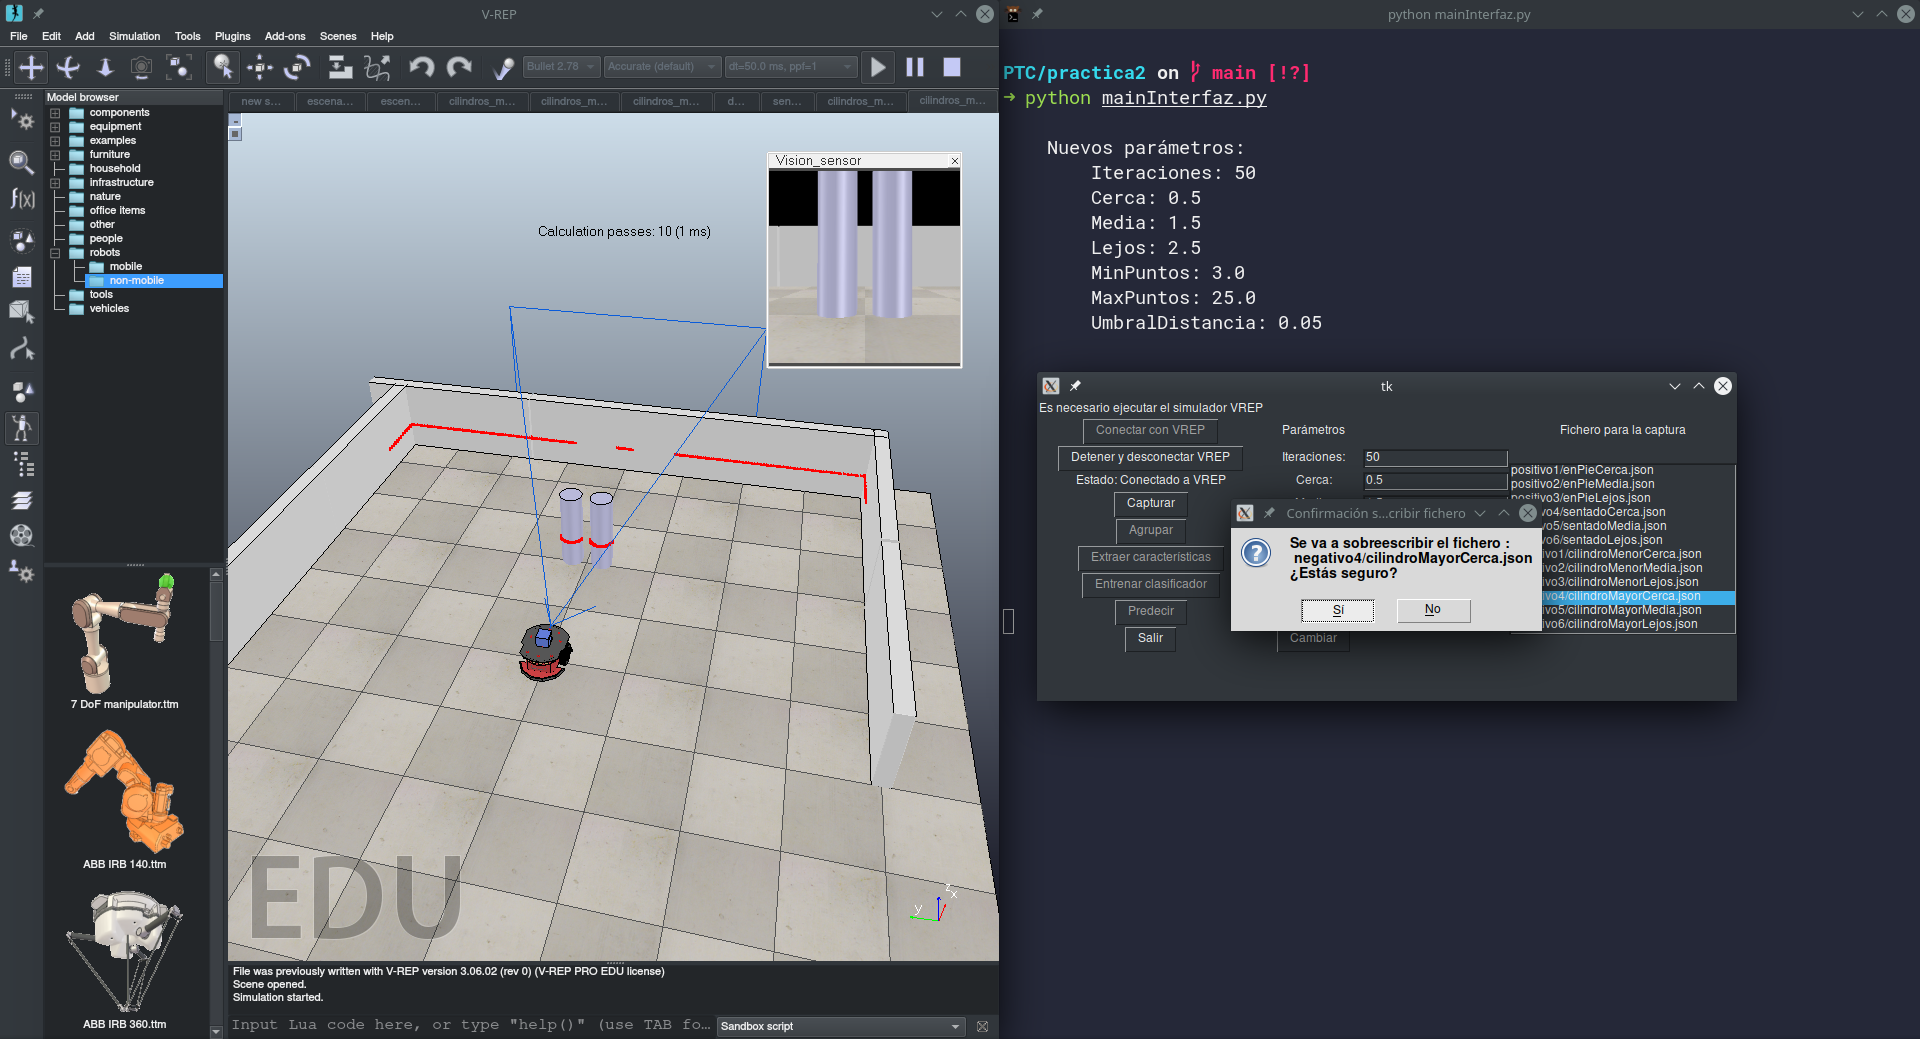
\includegraphics[width=\textwidth]{cilindro_m_cerca.png}
    \caption{Captura de datos con cilindro grande cerca.}
\end{figure}

\begin{figure}[H]
    \centering
    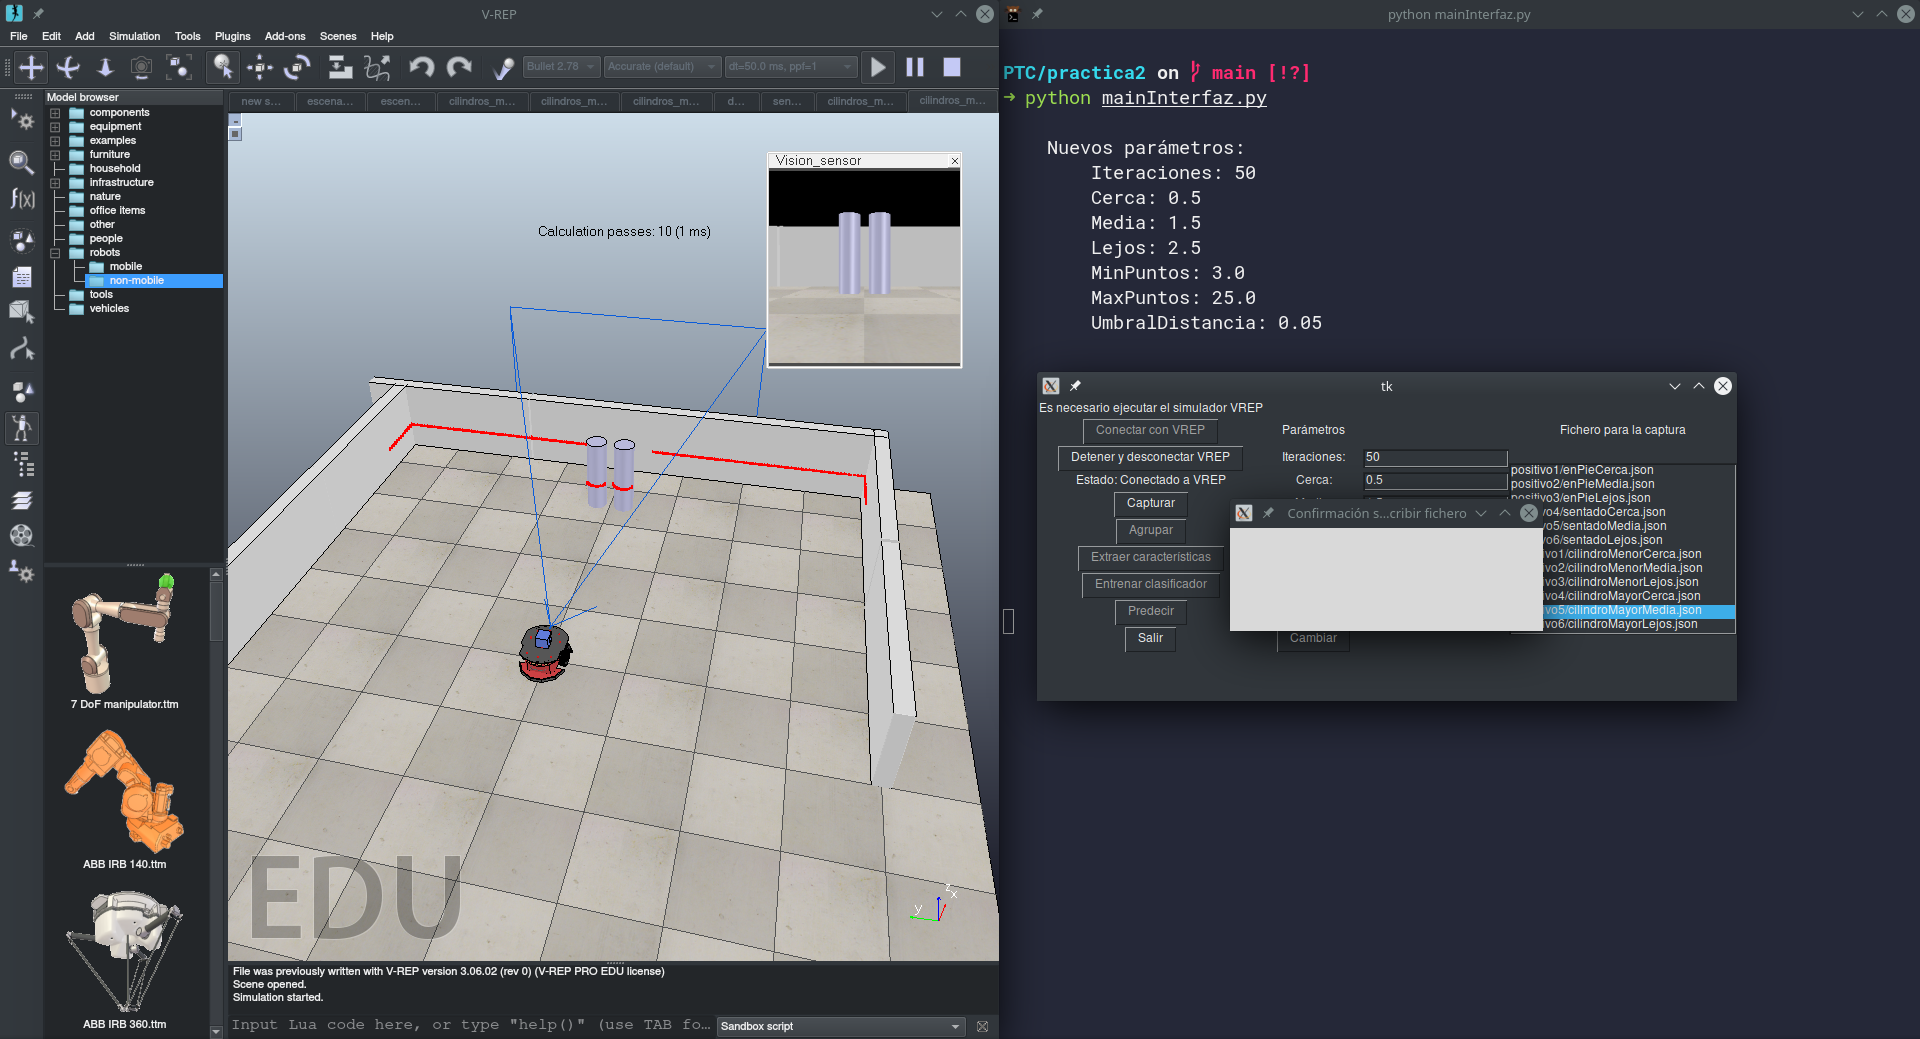
\includegraphics[width=\textwidth]{cilindro_m_media.png}
    \caption{Captura de datos con cilindro grande media.}
\end{figure}

\begin{figure}[H]
    \centering
    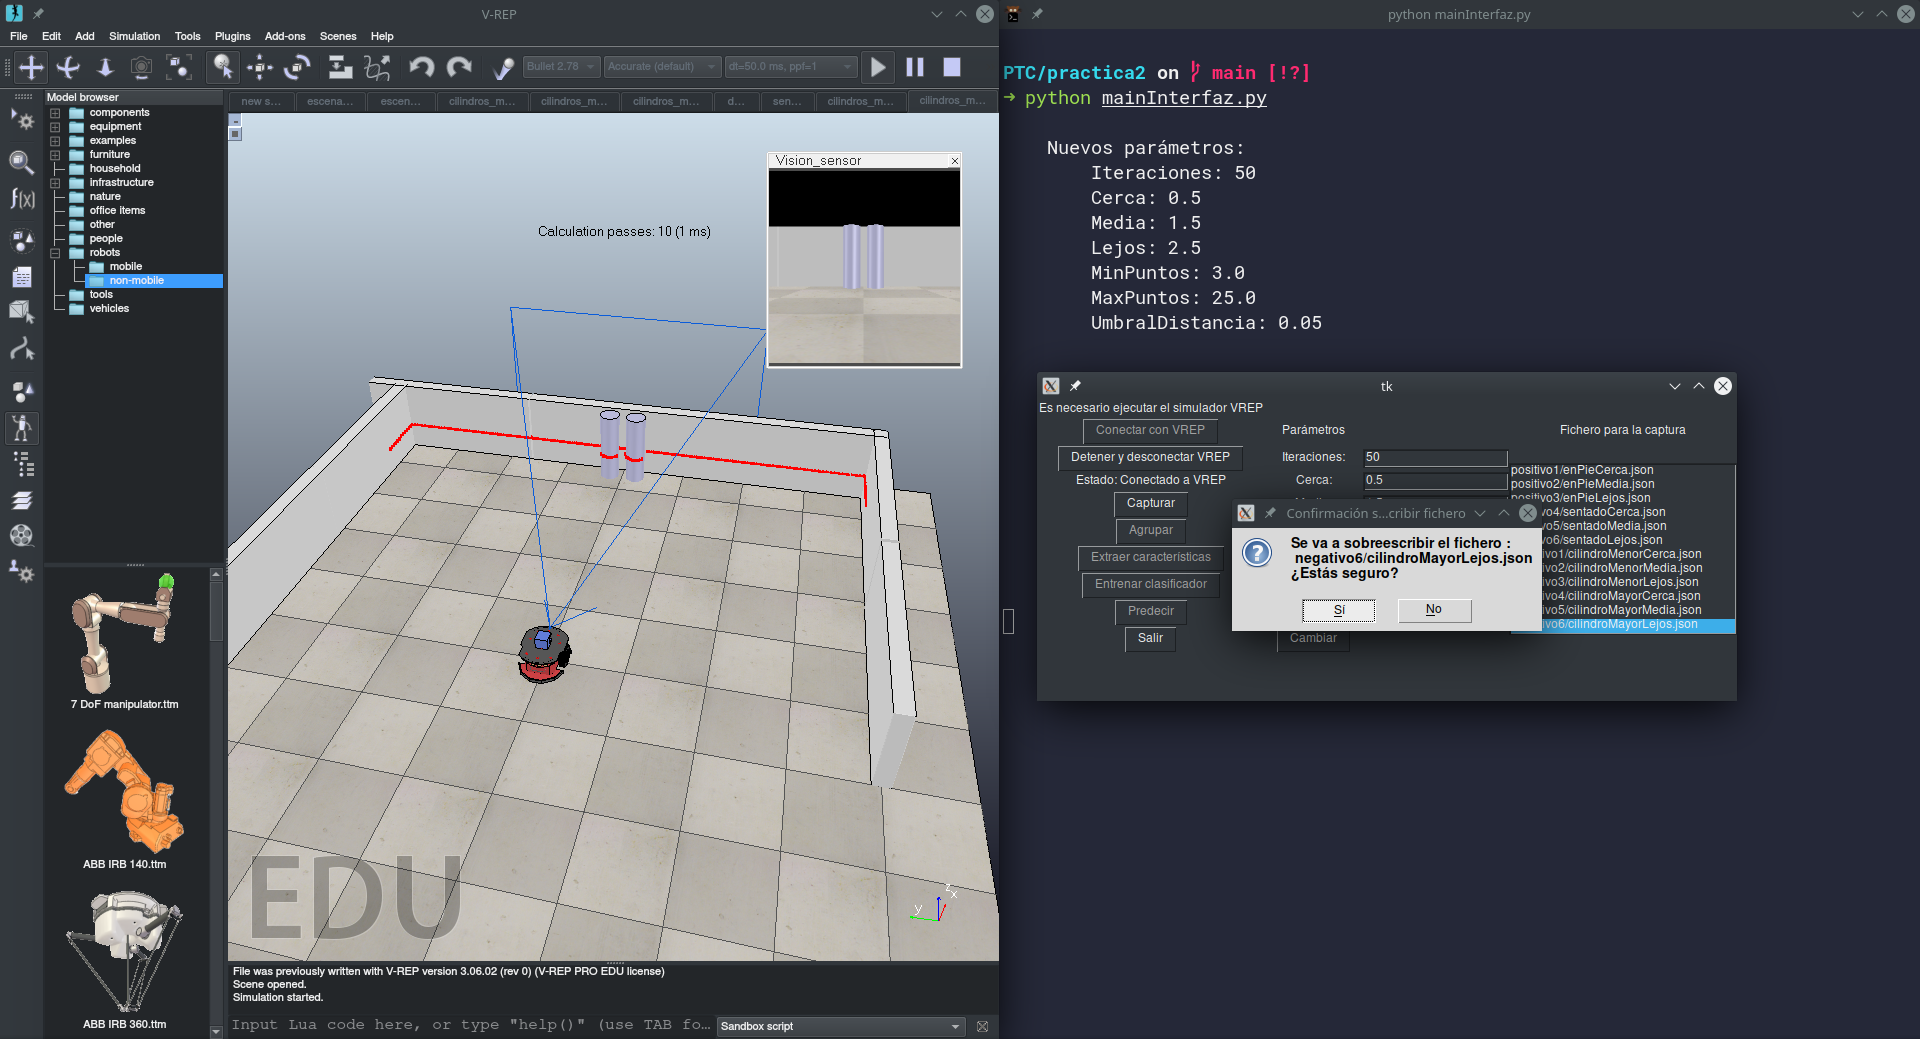
\includegraphics[width=\textwidth]{cilindro_m_lejos.png}
    \caption{Captura de datos con cilindro grande lejos.}
\end{figure}

\subsection{Resultados del aprendizaje de la SVM}

\begin{figure}[H]
    \centering
    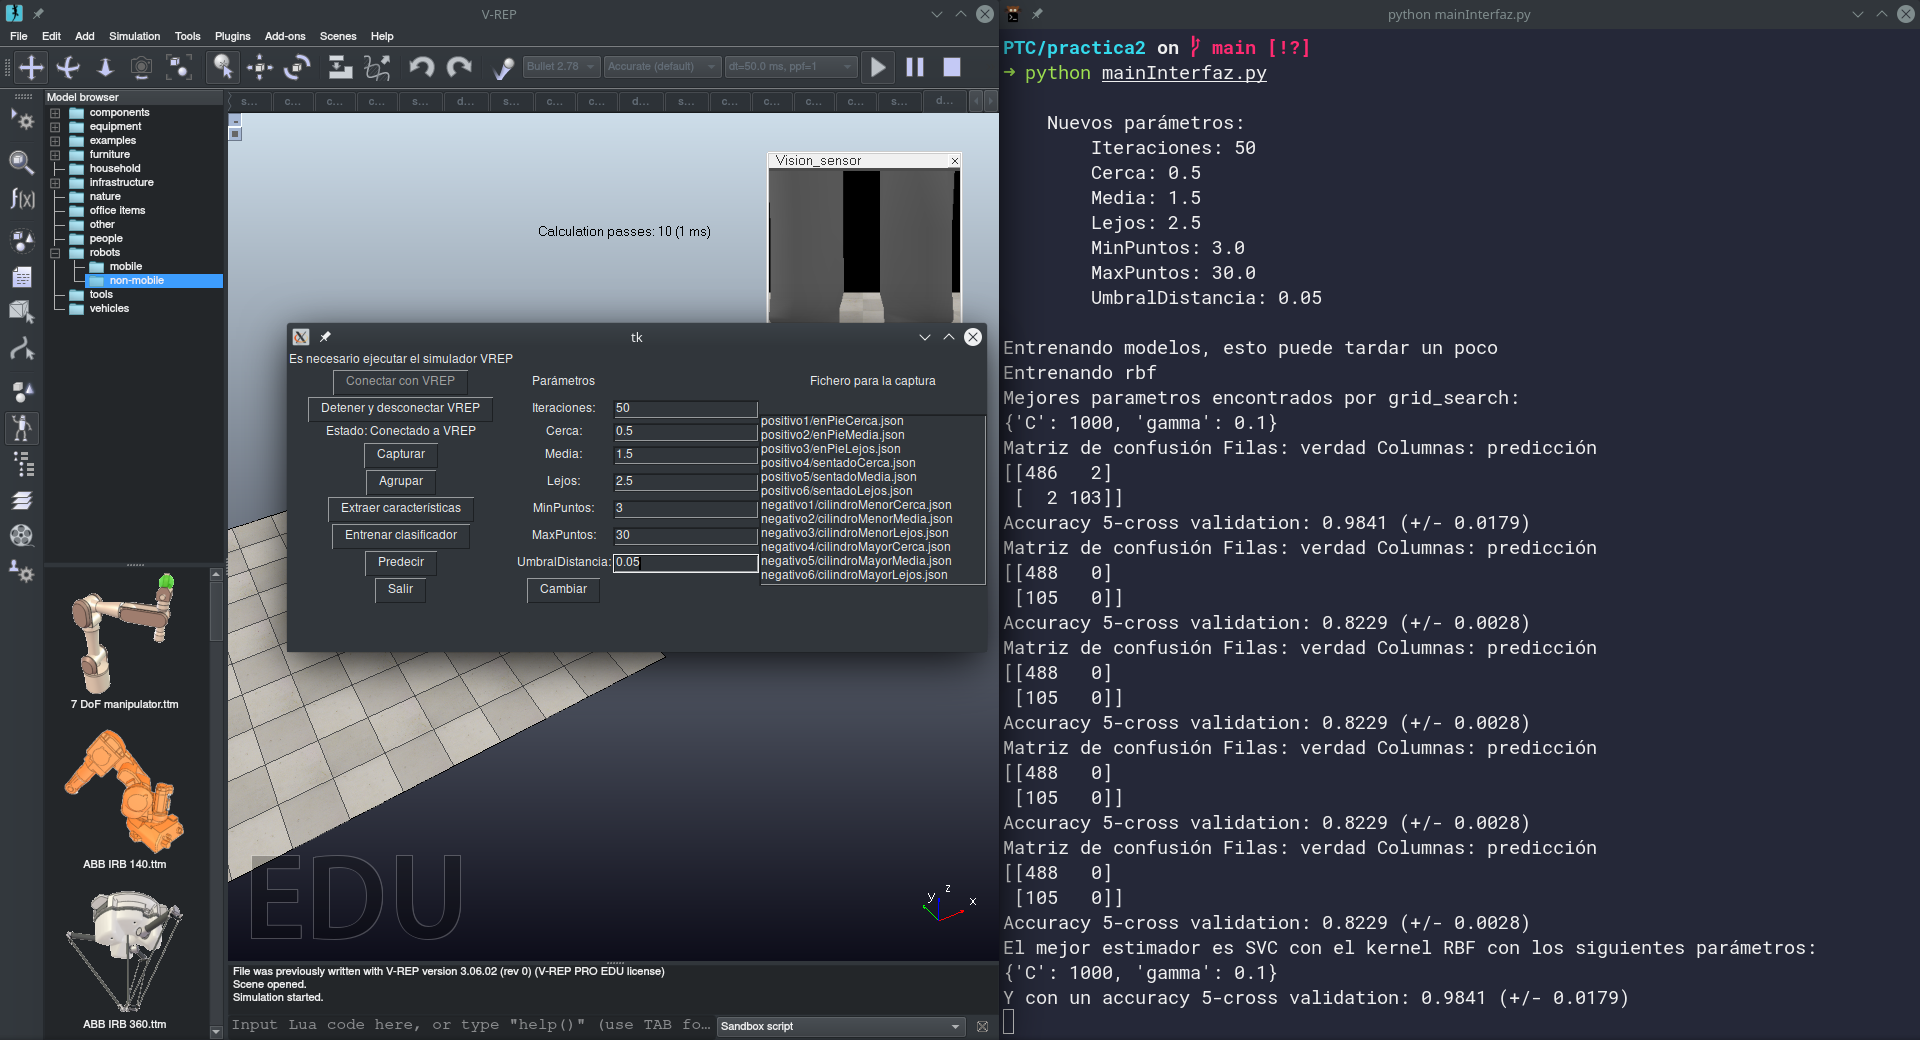
\includegraphics[width=\textwidth]{salida_entrenar.png}
    \caption{Salida tras entrenar el clasificador.}
\end{figure}



\begin{lstlisting}
Entrenando modelos, esto puede tardar un poco
Entrenando rbf
Mejores parametros encontrados por grid_search:
{'C': 1000, 'gamma': 0.1}
Matriz de confusión Filas: verdad Columnas: predicción
[[486   2]
 [  2 103]]
Accuracy 5-cross validation: 0.9841 (+/- 0.0179)
Matriz de confusión Filas: verdad Columnas: predicción
[[488   0]
 [105   0]]
Accuracy 5-cross validation: 0.8229 (+/- 0.0028)
Matriz de confusión Filas: verdad Columnas: predicción
[[488   0]
 [105   0]]
Accuracy 5-cross validation: 0.8229 (+/- 0.0028)
Matriz de confusión Filas: verdad Columnas: predicción
[[488   0]
 [105   0]]
Accuracy 5-cross validation: 0.8229 (+/- 0.0028)
Matriz de confusión Filas: verdad Columnas: predicción
[[488   0]
 [105   0]]
Accuracy 5-cross validation: 0.8229 (+/- 0.0028)
El mejor estimador es SVC con el kernel RBF con los siguientes parámetros: 
{'C': 1000, 'gamma': 0.1}
Y con un accuracy 5-cross validation: 0.9841 (+/- 0.0179)
\end{lstlisting}

\subsection{Resultados en escena de test}

\begin{figure}[H]
    \centering
    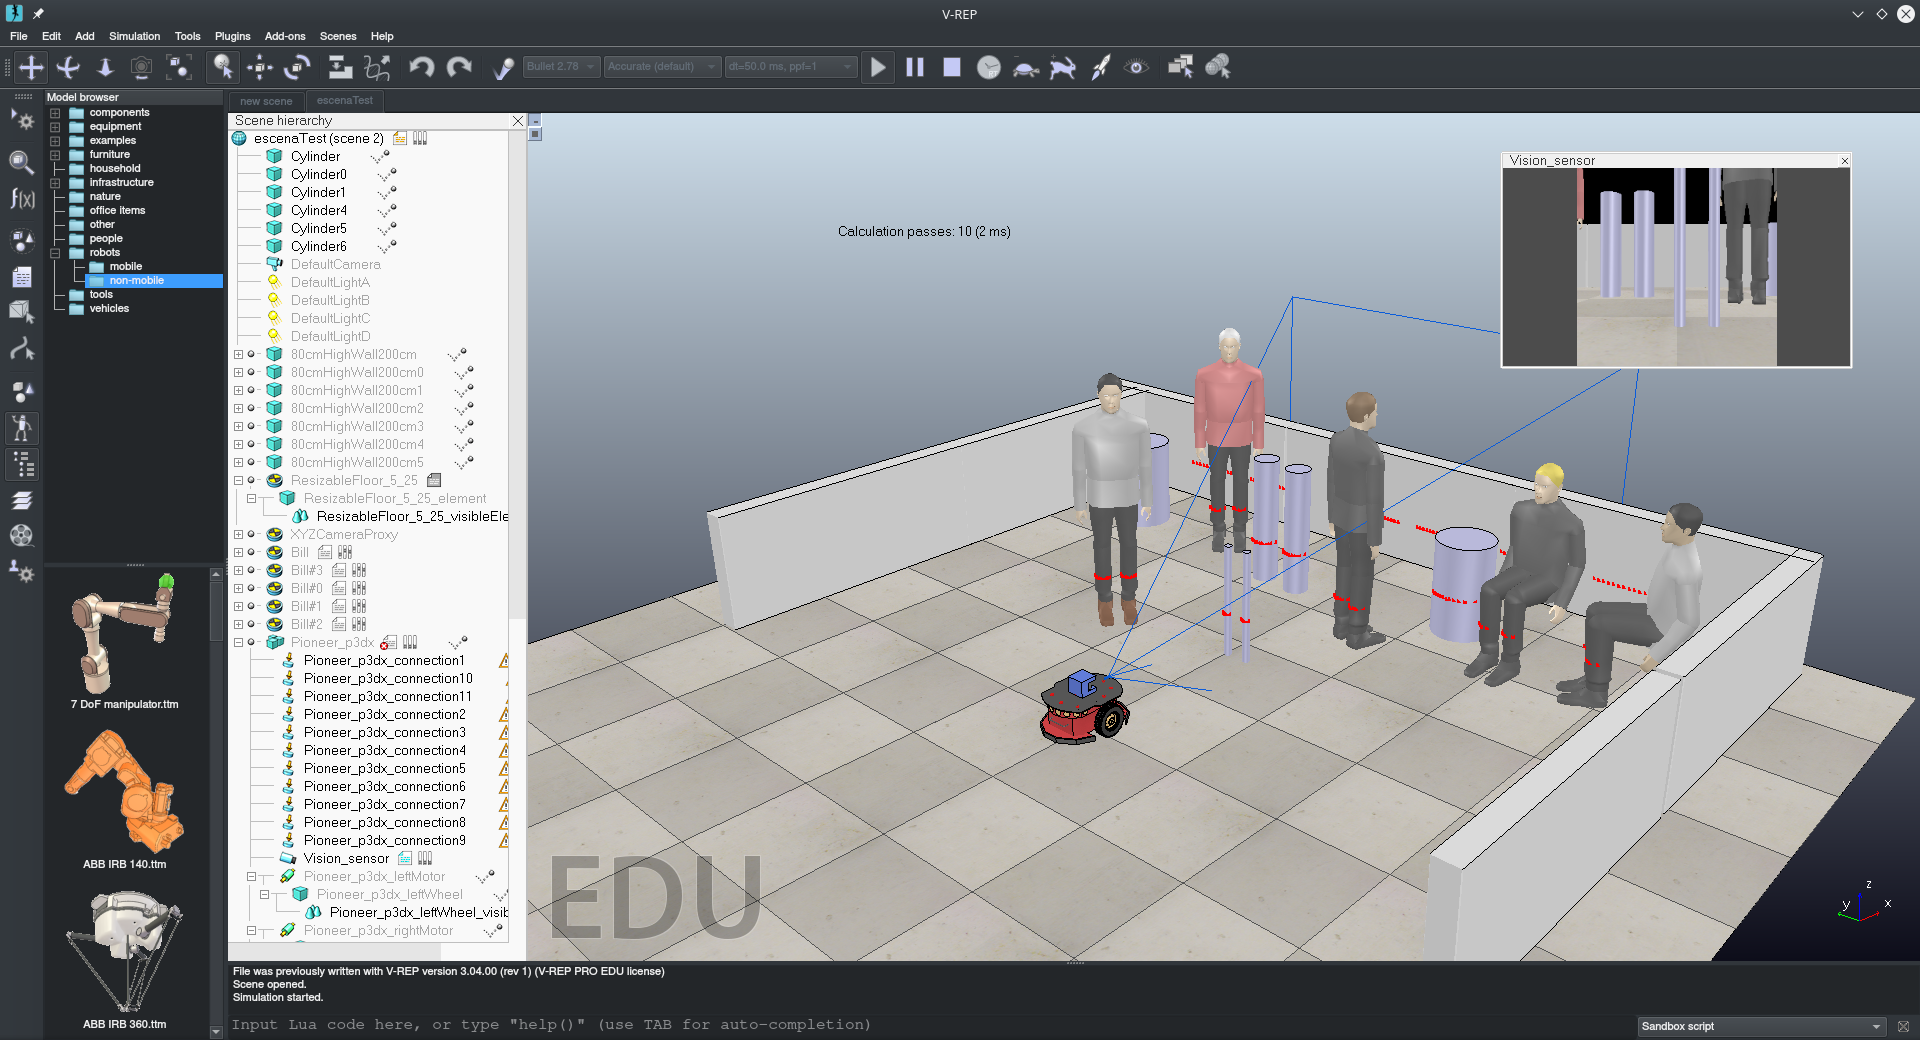
\includegraphics[width=\textwidth]{escena_test.png}
    \caption{Escena de prueba para predecir.}
\end{figure}

\begin{figure}[H]
    \centering
    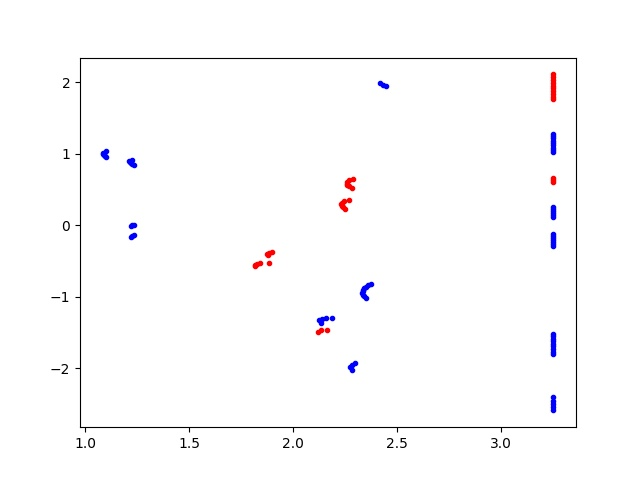
\includegraphics[width=\textwidth]{capturaTest.jpg}
    \caption{Resultados de la predicción.}
\end{figure}


% \begin{thebibliography}{9}
%
%
% \end{thebibliography}

\end{document}
